\documentclass[a4paper]{report}
\usepackage[utf8]{inputenc}
\usepackage{graphicx} % Required for inserting images
\usepackage{amsmath}
\usepackage{amssymb}
\usepackage{bookmark}
\usepackage{booktabs}
\usepackage{titlesec}
% \usepackage[T1]{fontenc}
% \usepackage{pgfplots} 
% \usepackage[myheadings]{fullpage}
\usepackage{tikz}
\usetikzlibrary{positioning}
\usetikzlibrary{calc} 
\usetikzlibrary{shapes.geometric}  % Required for regular polygons
\usetikzlibrary{decorations.pathmorphing}  % Enables zigzag paths
\usetikzlibrary{decorations.text}
\usetikzlibrary{decorations.markings}
\usetikzlibrary{intersections}
\usetikzlibrary{arrows.meta} 
\usepackage{hyperref}
\usepackage{float}
\usepackage{fancyhdr}
\usepackage{array}
% \usepackage{enumitem}
% \usepackage{changepage}
\usepackage{subcaption} % loads the caption package
\usepackage{import}
\usepackage{geometry}
\usepackage{adjustbox}
\usepackage[margin=1cm]{caption}
\usepackage[style=vancouver]{biblatex}
\usepackage{algorithm2e}
\usepackage[affil-it]{authblk}
\usepackage[symbol]{footmisc}

\renewcommand{\thefootnote}{\fnsymbol{footnote}}

%Algorithm2e settings
\LinesNumbered
\SetAlgoNoEnd
\SetAlgoVlined
\DontPrintSemicolon
\SetAlgoSkip{medskip}
\SetCustomAlgoRuledWidth{.7\linewidth}
\SetAlCapSkip{5mm}
% \SetFuncSty{\textcolor{blue}{\textbf{#1}}} 
% \newcommand{\mycapfn}[1]{\textcolor{blue}{\textbf{#1}}}\SetFuncSty{mycapfnt}
% \newcommand{\myargfn}[1]{\textcolor{green}{\emph{#1}}}\SetFuncArgSty{myargfn}
% \SetAlFnt{\texttt}

\addbibresource{all.bib}

\setlength{\parindent}{0px}
\pagestyle{fancy}

\geometry{
  a4paper,
  %total={170mm,257mm},
  left=25mm,
  right=25mm,
  top=20mm,
}

% Header and footer information
\fancyhf{}
% \setlength\headheight{15pt}
% \fancyhead[L]{} 
% \fancyhead[R]{}
\fancyfoot[R]{\thepage}

\newcommand{\HRule}[1]{\rule{\linewidth}{#1}}

\titleformat{\chapter}[display]%
{\bfseries\Large}%
{}%
{0ex}%
{\titlerule\vspace{1ex}\filleft}%
[\vspace{1ex}\titlerule]

% \title{Optimizing switch states in distribution grids}
% \author{Sidney Pauly\inst{1} \inst{2}\\ Supervisors: Dr. Nicol\'as Rubido\inst{1} Dr. Christian K\"ohler\inst{2}}
% \author{Sidney Pauly}
% \graphicspath{img/ABDN.png}

\begin{document}

\author{Sidney Pauly%
\thanks{Main author; \texttt{me@sidneypauly.me}}\\}
\affil{University of Aberdeen, Venios GmbH and Smart Infrastructure Limited}

\author{Dr. Nicol\'as Rubido%
\thanks{Supervisor; \texttt{nicolas.rubidoobrer@abdn.ac.uk}}}
\affil{University of Aberdeen, School of Natural and Computing Sciences}

\author{Dr. Christian K\"ohler%
\thanks{Supervisor; \texttt{christian.koehler@venios.de}}}
\affil{Venios GmbH}

\date{April 18, 2025}

% \date{Dated: \today}

% \begin{titlepage}
% 	\begin{center}
% 		\includegraphics[width=50mm]{img/ABDN.png}\\[.5cm]
% 		School of Natural and Computing Sciences\\
% 		\HRule{2pt} \\
% 		\LARGE \textbf{Optimizing switch states in distribution grids}
% 		\HRule{2pt} \\ [0.5cm]
% 	\end{center}
% \end{titlepage}

\title{\includegraphics[width=50mm]{img/ABDN.png}\\[.5cm]
		School of Natural and Computing Sciences\\
		\vspace{2.5cm}
		\includegraphics[width=50mm]{img/venios.png}\\[.5cm]
		\HRule{2pt} \\
		\LARGE \textbf{Optimizing Switch States in Distribution Grids}\\
		\vspace{3mm}
		\large Undergraduate Thesis
		\HRule{2pt} \\ [0.5cm]
		% \normalsize \today\vspace*{5\baselineskip}
		}%
		
\maketitle

\tableofcontents

\clearpage

\chapter{Introduction}

% \section{Introduction}

The electrical grid is divided into multiple levels. Whilst the higher levels of the grid connect
the entire countries the lower level grids go from house to house and are hence also called 
distribution grids. In the past electricity was mostly produced at higher levels in power plants
and consumed at the lower level. Also, the load patterns in the lower levels of the grid where
well predictable as they closely followed peoples work days. All this meant that a simpler setup
in the these girds was sufficient. In the past 20-30 this has changed. A lot of energy is now
being produced at these lower levels, e.g. through solar panels. Further, load patterns have shifted
as well with people charging their electric cars, heating with heat pumps and generally consuming
their energy at different times (e.g. because of home office)\autocite{venios}.
To fix load and instability issues arising
from this, there are broadly two options, either you build more physical infrastructure "blindly" to always
have a safe margin or you gather insight into the grid by measuring and simulating laods. This can either
be used in real time to actively control the grid or beforehand to have a better idea of load margins as well
as to more efficiently add new physical infrastructure. One active control measure that can be taken
to optimize load is by switching switches in the grid controlling how much of it is interconnected.
Generally a distribution grid connects up a few houses to a few streets depending on the region or country.
Each of these "grid islands" is connected up to the higher level through a transformer. By changing over
switches in the grid one can connect up these islands, making bigger grid areas or regroup certain parts
of these islands into neighbouring ones. Both can have effects on the grid in a non-linear complex way.\\
\\
The aim of this dissertation is to explore the effects switching switches has on the grid, by simulating them
and measuring effects on various grid load and stability quantities. This analysis will then be used to develop
predictive formulas, heuristics and algorithms to find improved switch states compared to the currently used
switch state.


\section{Existing Literature}

Within literature two research subjects exist that deal with switches in the
electrical grid: Optimal Transmission Switching (OTS)\autocite{ots_lit_review}
and Switch Allocation Problem (SAP)\autocite{switch_allociation_lit_review}.\\
\\
OTS is usually focused on transmission grids and aims to reduce the overall
operation costs by taking out certain transmission lines. It often also incorporates other grid control
mechanisms into the optimization. A key difference between OTS and the aim of this
work is that OTS generally avoids islanding completely, i.e. it only considers one big interconnected grid 
area. Also, because usually does not deal with the distribution grid, transfomers as the connection point
to the rest of the grid are generally not considered. 
Lastly within the context of OTS the main goal is to switch transmission lines,
meaning taking them out of use. Within the distribution grid switching is instead
primarily aimed at isolating different grid areas from each other or to connect
previously unconnected ones. Not using specific cables is not a major aim.\\
\\
SAP is focused on the distribution grid, however instead of asking which switches to switch
it asks where switches should ideally be installed to increase gird reliability and reduce costs.
SAP does not focus on the question of how the switches in the grid should
then be configured once they are in operation.\\
\\

A possible name for this problem
could be Optimal Switch State Problem (OSSP) or Optimal Switch Configuration Problem (OSCP).
Literature on OSSP or OSCP seems to be very limited. The only available
literature we are aware of are the works of
Kerzel et al.\autocite{optimal_switch_configuration} and
Wolter et al.\autocite{meshed_grids}. Both of these consider German grids, 
with their relatively high count of producers in the distribution grid. 




\section{The need for a switch state score}

To compare switch states against each other a switch state score is required. 
Within the OTS and SAP literature a monetary cost is commonly used. It either
calculates the cost of outages in case of the SAP\autocite{switch_allociation_lit_review}
or by calculating the overall cost
of energy generation in the case of OTS\autocite{ots_lit_review}. The two papers
looking into OSSP or OSCP also use a cost function, here the cost of expansion
is considered, i.e. how much it would cost to add new prosumers to the grid
for different switch states.\\
\\
Directly optimizing for monetary cost is not desirable within the scope of this
project. Firstly, it is hard to estimate what costs are associated
to for example cable and transformer wear. Further there might even
be conflicts between short term costs and long term costs, e.g.
fewer line losses might be incurred by running the transformer at
a higher utilization, which would in turn incur long term maintenance costs.\\
This project aims to develop a general switch state optimization framework
applicable to all of Venios' customers. Different grid operators
in different regions, might pay different amounts for components, maintenance, electricity
or penalty charges.\\
Lastly this optimizer might be used in conjunction with different optimizers.
If a grid operator for example has to connect a new prosumer to their grid,
then different options might be weight depending on how they could somehow
accommodate the new prosumer. If the switch state optimizer is able
to return a result where the additional prosumer can be connected without
any physical grid expansion and other options do require physical grid expansion, then
using switching will likely always be cheaper\autocite{venios}. 
This is to highlight that an optimizer that optimizes for operational
grid parameters will be easier to accommodate then one that already optimizes
for cost.\\
\\
As there is no precedent for non-monetary cost functions for OSSP or OSCP adjecent
problems we introduce our own score within this work. The main goal of this score
is to balance different operational parameters and unify them into a single number.
As different grid operators will have different requirements an additional aim
is to have this score be easily fine tuneable by the grid operator themselves.
To achieve this we propose a scoring equation
that uses operational grid quality parameters already known and
used by the grid operators. The proposed equation also enables 
the grid operator to weigh these different aspects, thus enabling them to fine
tune the score to their specific needs.\\


\section{Study case}

% Applied to venios customers
% As such done on real grids, instead of sythetic examples.
% Specifically this is being done on entire grid areas, thus isntead of disconnecitng
% lines we start from the existing grid structure and reconfigure it for better results
% No other load shedding mechanisms, or other control mechanisms
% Fixed generation and consumption (this si largly due to regulations)
% This is to be applied in an operational context: i.e. we take the current state
% of the grid with its current generation and topology and determine the best switch
% state within. Defining the "best" switchstate is not straightforward as switching
% impacts different parameters in the gird in different ways. Thus different
% optimization goals are presented, which can then be selected as needed or prefered
% in the operational context

% One restriction being imposed witin this work is single feed in, meaning that only
% one transformer supplies a given distribution grid. 

As a study case the grid of one of Venios' Swiss customers will be used. 
They operate over a thousand
low voltage grids in rural, suburban and urban areas\autocite{venios}. 
A grid in this context is a gird area containing a transformer and supplying
a neighbourhood of 60 or more buildings\autocite{venios}. These grids have switches
within and switches connecting them to neighbouring grids. Within the standard
switch state (SSS), all switches to other grids are open. This switch state is
used under normal operating conditions\autocite{venios}. To test the effect of switching
we select geographical boxes within the grid operators' region containing 5-10 grids each.
We then examine different switching states and apply different optimizers with the goal
of finding switching states with improved operational parameters over the SSS.\\
\\
The laws in Switzerland mandate equal and continuous access to the grid for every household.
Further Switzerland allows feed-in by private households with a right to sell guaranteed
for small producers\autocite{venios}. The implications of this are that continuous supply
and continuous feed-in has to be guaranteed at the distribution grid level with penalties
imposed in case of violation. Subsequently, any disconnection of grid members needs
to be avoided and mandated load shedding is both costly and needs to be distributed
over grid customers equally\autocite{venios}. All of this combined presents a strong
argument for switch state optimization as it poses an opportunity to improve grid operational
parameters with almost no costs to the grid operator.

\chapter{Theory}

% \import{sections/theory/}{ac-basics.tex}

\section{AC Basics}

To the grid operates on alternating current, thus an
understanding of the underlying formulas governing ac systems will be required to analyse it. \\
In an AC system both current and voltage oscillate. This can be generally described using the following two equations:

\begin{equation}
    V(t) = V_m cos(\omega t + \theta_V)
    \label{eq:ac:voltage_ac}
\end{equation}

\begin{equation}
    I(t) = I_m cos(\omega t + \theta_I)
    \label{eq:ac:current_ac}
\end{equation}

where $V_m$ and $V_m$ are the magnitudes of voltage and current,
$\omega$ the angular velocity of the oscillations and $\theta_V$ and $\theta_I$
the phase offset of Voltage and current.\\
Power as a function of time can then be defined as:

\begin{equation}
    P(t) = V(t)I(t)
    \label{eq:ac:power_t}
\end{equation}

Expanding this leads to the following expression:

\begin{equation}
    \begin{aligned}
        P(t) = \frac{1}{2} V_m I_m (\cos (\theta_V-\theta_I) 
        + \cos(2(\omega t + \theta_V))\cos(\theta_V-\theta_I)
        + \sin(2(\omega t + \theta_V))\sin(\theta_V-\theta_I))
    \end{aligned}
    \label{eq:ac:power_ac_long}
\end{equation}

which can be simplified using

\begin{equation}
    \begin{aligned}
        &\text{Impedance angle}: \quad  \theta &= \theta_V - \theta_I \\
        &\text{Root mean square of } V: \quad  |V| &= \frac{V_m}{\sqrt{2}} \\
        &\text{Root mean square of } I: \quad  |i| &= \frac{I_m}{\sqrt{2}} \\
    \end{aligned}
    \label{eq:ac:power_def}
\end{equation}
         
\begin{equation}
    \begin{aligned}
        P(t)   &= P_R(t) + P_X(t)\\
        P_R(t) &= |V||I| \cos(\theta) (1 + \cos(2(\omega t+\theta_V)))\\
        P_X(t) &= |V||I| \sin(\theta) (1 + \sin(2(\omega t+\theta_V)))\\
    \end{aligned}
    \label{eq:ac:power_react_and_capacitive}
\end{equation}

If we are interested in steady state scenarios, then we can assume $\omega$ and $\theta_V$ 
to be constants. Over longer periods of time the average of $\sin(A t + B)$ and $\cos(A t + B)$ are 0.\\
We can thus simplify $P_R$ and $P_X$ further:

\begin{equation}
    \begin{aligned}
        P_R(t) &= P = |V||I| \cos(\theta)\\
        P_X(t) &= Q = |V||I| \sin(\theta)\\
    \end{aligned}
    \label{eq:ac:power_react_and_imag}
\end{equation}

It is handy to define these as the real and imaginary parts of a complex number:

\begin{equation}
    \begin{aligned}
        S     &=  V I^*\\
        S     &= P - iQ\\
        Re(S) &= P\\ 
        Im(S) &= Q
    \end{aligned}
    \label{eq:ac:complex}
\end{equation}

\begin{figure}[H]
    \centering
    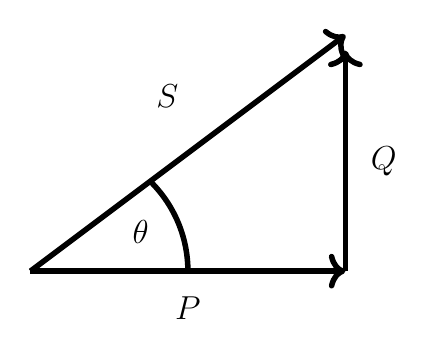
\begin{tikzpicture}[scale=2]
    \draw[->, line width=.7mm] (-1, 0) -- (1, 1.5) node[pos=.65](s){};
    \draw[->, line width=.7mm] (-1, 0) -- (1, 0) node[pos=.5](p){}; 
    \draw[->, line width=.7mm] (1, 0) -- (1, 1.4) node[pos=.5](q){};  

    \draw[line width=.7mm] (0, 0) arc (0:45:.8);

    \node[text width=2cm] at (s)[above] {\large $S$};
    \node at ($(q) + (.1, 0)$)[right] {\large $Q$};
    \node at ($(p) + (0, -.1)$)[below] {\large $P$};
    \node at (-.3, .25) {\large $\theta$};
\end{tikzpicture}
    \caption{
        The power triangle showing the relation between complex power $S$,
        real power $P$, reactive power $Q$ and the power angle $\theta$.
    }
    \label{fig:ac:power_triangle}
\end{figure}

To describe an AC grid we also need to introduce a complex version
of Ohm's law:

\begin{equation}
    V = ZI
    \label{eq:ac:ohm_complex}
\end{equation}

where $Z$ is impedance which is defined as:

\begin{equation}
    Z = R + iX
    \label{eq:ac:impedance}
\end{equation}

where $R$ is resistance and $X$ is reactance. Reactance measures how much
energy will be stored in the cable within a current cycle due to a magnetic
field being created\\

Lastly we can also define an ac-equivalent for conductance, which is called admittance $Y$:

\begin{equation}
    Y = 1/Z
    \label{eq:ac:admittance}
\end{equation}

\section{Power flow}

To formulate the power flow equation, we can start form the general assumption
that the current entering a node has to equal the current exiting it, i.e.
there is conservation of charges.\\
There are two sources for current through a node:

\begin{itemize}
    \item Current due to production/consumption at the node
    \item Current from or to other nodes
\end{itemize}

The current due to production/consumption at node $i$ itself is
obtained by considering
the complex power \autoref{eq:ac:complex}:

\begin{equation}
    \begin{aligned}
        S_i     &= V_iI_i^*\\
        I_i     &= \frac{S_i^*}{V_i^*}.
    \end{aligned}
    \label{eq:pf:current_due_to_prosumer}
\end{equation}

Defining the current due to the other nodes requires the use of
Ohm's law (\autoref{eq:ac:ohm_complex}).
The current flowing from the current node (node $i$)
to one of the adjacent nodes (node $j$) will be a result of the
voltage difference between the current node and its neighbour:

\begin{equation}
    \begin{aligned}
        \Delta V_{ij} &= Z_{ij} I_{ij} \\
        I_{ij}        &= (V_i - V_j) Y_{ij},
    \end{aligned}
    \label{eq:pf:neighbour_current}
\end{equation}

where $Y_{ij}$ is the admittance between nodes $i$ and $j$.
Summing over \autoref{eq:pf:neighbour_current} for all neighbours of $i$:

\begin{equation}
    \begin{aligned}
        I_{i} &= \sum_{i \ne j}^N (V_i - V_j) y_{ij}\\
              &= V_i \sum_{i \ne j}^N y_{ij} - \sum_{i \ne j}^N V_j y_{ij}.
        \label{eq:pf:current_at_node}
    \end{aligned}
\end{equation}

The case $i = j$ can be ignored as $\Delta V_{ii} = 0$.\\
\\
Equating the two sources for current \autoref{eq:pf:current_due_to_prosumer}
and \autoref{eq:pf:current_at_node} results in the power flow equation:

\begin{equation}
    \begin{aligned}
        V_i \sum_{i \ne j}^N Y_{ij} - \sum_{i \ne j}^N V_j Y_{ij} = \frac{S_i^*}{V_i^*}.
        \label{eq:pf:pf_eq_large}
    \end{aligned}
\end{equation}

One further simplification can be employed by using an admittance matrix.
The elements of which are:

\begin{equation}
    y_{ij} =
    \begin{cases}
        \sum_{i \ne j} y_{ij} & \text{for} \ i = j\\
        -Y_{ij}               & \text{for} \ i \ne j.
    \end{cases}
    \label{eq:pf:admittance_matrix}
\end{equation}

Thus equation \ref{eq:pf:pf_eq_large} can be further simplified:

\begin{equation}
    \sum_{j=1}^N V_j y_{ij} = \frac{S_i^*}{V_i^*}.
    \label{eq:pf:full_pf_eq}
\end{equation}

Note the change from using admittance $Y_{ij}$ to the admittance matrix
elements $y_{ij}$.\\
\\
This power flow equation is non-linear, which thus necessities the use of a computational
solver. Two such solvers, are introduced in \autoref{sec:methods:pf}\\
\\
To simulate the grid a way to solve the power flow problem is needed. 
To solve power flow we assume,
that we know all the production and consumption for all prosumers,
as well as the voltage at the so-called slack
node (for this node the consumed/produced power is not known). Using a
power flow solver we can then determine the voltage
at all the other nodes in the grid as well as the power at the slack 
node. This information then also suffices to determine
the currents through all cables. Taken together these quantities 
give a fairly good overview of how the grid performs.

\begin{figure}[H]
    \centering
    \begin{tabular}{ l|r r r }
        Node type          & Power     & Voltage & Count \\ 
        \midrule
        \textbf{Slack}     & Unknown   & Known   & 1     \\  
        \textbf{Prosumer}  & Known     & Unknown & n    
    \end{tabular}
    \caption{
        Types of nodes relevant to solving power flow.
    }
\end{figure}


\section{Graph theory}

The electrical grid can be represented as a graph. 
In a graph theory a graph is defined as a set of nodes and edges. A node
is some point in the graph, whilst an edge is a connecting element between exactly
two nodes.\\
\\

The simplest form of a graph is where the nods and edges do not have
any additional information attached to them and the edges are bidirectional.
I.e. the edge $A \to B$ is the same as the edge $B \to A$. Even though the setup
of such a graph seems simple, there are numerous metrics and complicated questions
that can be asked at this level. For example trying to find the quickest way between
two points in a graph is already a non-trivial problem that has its own class of algorithms
(e.g. A*, etc.). In the context of this project graph-theory becomes important in two ways.
Firstly it informs how the grid data is represented and processed and secondly it can
be used to classify certain configurations of the grid, through graph measures.

\subsection{Grid data representation}

In the most fundamental terms the grid can be represented as nodes, which are the 
producers or consumers (also called prosumers) and cables, which are the edges.
The prosumers have a production or consumption capacity $S_i$ (complex power see eq. \ref{eq:ac:complex}).
The cables have an admittance $Y_{ij}$ (see eq. \ref{eq:ac:admittance}).\\
\\
3 ways to represent the graph data will be subsequently used. 
Each records the full information of the graph, but
has different advantages and disadvantages. Note that the examples shown below all record
the admittance of each cable in addition to the info that the cable exists. Sometimes
this info is not need in which case it can be omitted and the representation further simplified/

\subsubsection{Edge list}

In edge list representation there is an entry for each edge in the graph in form of a vector:

\begin{equation}    
    \mathfrak{E_{ij}} = (i,\ j,\ Y_{ij})
\end{equation}

here $i$ and $j$ are the index of node A and B connected by the edge and
$Y_{ij}$ the admittance of the edge (cable).
For sparse graphs (graphs where only a handful of all possible edges $\mathfrak{E_{ij}}$ exist), this method
of storing the graph data is very efficient as only as many entries as cables are required. The disadvantage
algorithmically is that finding a specific connection between is not so efficient as it has to be searched for amongst
all entries. E.g. to look up admittance between nodes a and b that specific edge has to be found.

\subsubsection{Matrix form}

In matrix form each row and column represents a node. Each entry in the matrix is the admittance between nodes $i$ and $j$.
If the admittance is not to be recorded than if a node exists the entry can be set to 1 and if not to 0 instead:

\begin{equation}
    Y =
    \begin{pmatrix}
        Y_{11} & Y_{12} & ... & Y_{1n}\\
        Y_{21} & ...    & ... & ...   \\
        ...    & ...    & ... & ...   \\
        Y_{n1} & ...    & ... & Y_{nn}\\
    \end{pmatrix}
\end{equation}

As the cables in a grid are symmetrical (admittance is the same for current from a to b as it is form b to a), 
the matrix is symmetrical as well: $Y_{ij} = Y_{ji}$. Further in pure graph representation all diagonal elements are
zero as there are no cables running in a loop starting and ending at the same node.\\ 
One big advantage of this representation is that it allows for quick lookups, i.e. if one needs the admittance between nodes a and b
one can simply look up that entry in the matrix.\\
A closely related matrix is the admittance matrix, here the diagonal elements are populated with the
so called self-admittance, which consist of the sum of admittances to the neighbouring nodes:
\begin{equation}
    Y_{ii} = \sum_{i \ne j} Y_{ij}
\end{equation}

The admittance matrix is useful as it can be directly used in some mathematical
or physical formulas like Ohm's law:

\begin{equation}
    V = YI
\end{equation}

The disadvantage of this form of representation is that it is very space inefficient, as it requires
$N^2$ entries (where $N$ is the number of nodes). Especially for sparse graphs a lot of these entreis contain
zeros and are thus redundant. This drawback in memory and iteration efficiency
can be mitigated by clever data structure arrangement, which will be discussed later. 

\subsubsection{Node representation}

In the node representation the graph is represented by the connections
each node has and the admittance to each other node:

\begin{equation}
    \mathfrak{N_i} = \sum_{i \ne j, Y_{ij} > 0} (j, \ Y_{ij}) 
\end{equation}

This representation is especially useful for things like flooding algorithms where it is
relevant to know which nodes can be reached from any given node in question. 

\subsection{Graph measures}

\chapter{Methods}

\section{Data available through VEP}

The \textbf{V}enios\textbf{E}nergy\textbf{P}latform is a cloud application
developed and hosted by Venios. The customers are grid operators who can use
it to visualize the grid, track real time data, have it predict 
operational parameters such as prosumer loads and control the grid.
The long term aim of this project is to develop an algorithm that takes in
congested grid areas as its input and advises VEP on possible improved
switch states and their effects. This dissertation aims to implement the first step of this
process by taking in grid data from VEP and analysing it, trying to figure out
improved grid configurations. Data obtained for this project from VEP can broadly
be categorized
into topological and load profiles. Whilst the former is anything having to do with
the grid structure, its geographical location and its operating parameters the later
are production or consumption values over time for each of the prosumers.\\
All data is obtained over Venios' API, in json format. This means any
grid area of any VEP customer can be used for this analysis just by changing out
the request parameters and use of the relevant authorization tokens for that customer.
No code changes are required. This approach has the added advantage that any customer grid
data is only stored in memory and only temporarily on the machine running the analysis. This
has data privacy advantages.

\subsection{Topological grid data}

The grid data coming from VEP contains edges and nodes.
The subtypes with relevance to this work are listed in tables \ref{table:vep:nodes} and
\ref{table:vep:edges}\\
\\
\begin{figure}[H]
    \begin{tabular}{l p{3cm} p{8cm}}
        Name & Power production/consumption & Description\\
        \hline
        Domestic prosumer & Consumes power & A household consuming power. Power is mainly consumed in the morning and evenings when people are home\\
        Industry prosumer & Consumes power & A store or factory. Power is mainly consumed during work hours\\
        Solar panel       & Produces power & Produces power based on sunlight, thus most power produced in the summer at mid-day\\
        Other prosumers   & Produces and consumes power & Other prosumers, like electric car chargers, batteries, heat pumps, etc. These can have a range of load patterns\\
        Any other node    & None           & Any other node acting as a junction, busbar or other. As they all do not consumer or produce power they are only relevant as so far as they act as junctions for cable connections
    \end{tabular}
    \caption{Node types relevant to this work}
    \label{table:vep:nodes}
\end{figure}

\begin{figure}[H]
    \begin{tabular}{l p{10cm}}
        Name & Description\\
        \hline
        Cable & Cables have impedance and a physical length\\
        Transformer & Connects a grid to a higher voltage level. Main feed-in point in a low voltage grid\\
        Switch & An edge that can be interrupted. Modelled with no impedance and no physical length\\
        Any other & Other miscellaneous edge not modelled with physical length or impedance. Usually connects nodes within a substation or electrical cabinet.
      \end{tabular}
    \caption{Edge types relevant to this work}
    \label{table:vep:edges}
\end{figure}

A good dataset for validation and comparison is the SimBench data set. It is a set of
gird data provided by the University Kassel. The dataset aims to model typical German
grids in rural and urban environments. It was specifically designed to include a higher
number of renewables in the low voltage level, like solar panels\autocite{simbench}. These
simbench grids can be also imported in VEP and where thus used as the initial validation case
for this work.\\

Figure \ref{fig:vep:simbench_node_types} shows one of these Simbench grids ("1-LV-rural1"). 
Within VEP this grid is modelled with 553 edges and 553 nodes. A lot of these nodes are there to model
internals like bus bars or protective switch setups. For power flow and for analysing
switch states these nodes can be merged down to 96 with 95 edges running between them. 
The exact method to do so will be explained in the data preparation section. These numbers of nodes
are typical for German grids\autocite{venios}.

\begin{figure}[h]
    \includegraphics{img/simbench/layout.png}
    \caption{
        Non-geographical representation of the SimBench "1-LV-rural1"
        grid\autocite{simbench}. Layout produced with
        Kamada-Kawai layout algorithm\autocite{kamada_kawai}.
        Nodes with connected transformers are shown
        in \textbf{grey}, households with solar panels in \textbf{green}
        and normal households in \textbf{red}. Only cables with non-zero impedance shown, any nodes
        connected by zero impedance cables have been merged.
    }
    \label{fig:vep:simbench_node_types}
\end{figure}

% The grouping into grids
% Outer world (for geographical locations)
%   Nodes
%   Edges
% Inner world (conducting)
%   Nodes (simple, prosumer, slack)
%   Edges (switches, simple, with impedance, transformers)
% Standard switchstate

\subsection{Grid Load}

To simulate the grid adequately, production and consumption values for
each of the prosumers is needed. VEP provides various different models
to do so ranging form standard load profiles (standardized curves which are adjusted
according to the prosumer's parameters), neural network models trained on historic data,
weather forecast based models, and actual real time measurement values\autocite{venios}.\\
\\
Within real low voltage girds, the data available will often be spotty. Not all prosumers
have measurement devices and their measurement frequency is often limited. The most accurate
load modelling data is therefore often a mixture of the sources mentioned above.\\
\\ 
For this work all load time series will be obtained from Venios through its API. Venios works
closely with the grid operators to make sure these timelines most closely resemble the conditions
in the real grid. This important as these values are being used to monitor the grid and in some
cases trigger active control measures\autocite{venios}. Within this work it is assumed that the data
available through the API is the best data available, which closely resembles the actual grid load.
Any switch states and their effects on grid parameters will be tested against this data. It can
thus be reasonably assumed that any improvements seen based on this data translate reasonably well
into the real world. 

\begin{figure}[H]
    \begin{subfigure}{.5\textwidth}
      \centering
      \includegraphics[width=\linewidth]{img/simbench/load_profile_household.png}
      \caption{}
      \label{fig:vep:load_profile_household}
    \end{subfigure}%
    \begin{subfigure}{.5\textwidth}
      \centering
      \includegraphics[width=\linewidth]{img/simbench/load_profile_solar.png}
      \caption{}
      \label{fig:vep:load_profile_solar}
    \end{subfigure}
    \caption{Power produced/consumed by a household (a) and a solar panel (b) within a SimBench grid at different times of day and at different times of year. Data is generated by a standard laod profile model within VEP and obtained over API\autocite{venios}}
    \label{fig:vep:load_profiles}
\end{figure}

Figure \ref{fig:vep:load_profiles} shows example load data obtained from VEP. It can be seen
that power production and consumption varies, widely throughout the day and the year. As a result the grid
might act very differently depending on the season and time. An important question to answer is therefore if
there are swtichstates that are generally better or if the best switch state is highly dependent on
time.\\
\\
Often switches within the grid can only be operated manually\autocite{venios}. Therefore, changing the grid configuration is linked to
some effort and cannot be done very often. If it turns out that there are switch states that are consistently better
a new and improved permanent switch state could be considered. If the best switch state is
however dependent on time, then depending on the scale of improvement, remotely controlled switches might be a worthwhile
investment.

\section{Power flow algorithms}\label{sec:methods:pf}

% Mention that the faster we can run power flow the more data can be collected later -> a main goal
% is to make power flow as fast as possible
% Validation:
%   1. Comparision with results obtained by book
%   2. Comparision with vep results?
% Gauss-Seidel
% Newton-raphson
% python-c adapter
% sparse matricies optimization
% Show performance of different methods over grid size?

To solve the power flow equation \ref{eq:pf:full_pf_eq} a numerical solver
is required\autocite{power_system_analysis}. In the context of this analysis
a vast number switch states have to be explored. The more swtichstates
can be explored in the same amount of time the better. Thus, a fast power flow
solver is required. There are numerous solvers power flow with different speed
and versatility tradeoffs\autocite{pf_methods_comparison}. Some methods might
only work on specific grid topologies like radial topologies, some other methods
might require the network to have decoupled real and reactive power flows to work.
The Gauss-Seidel and Newton-Raphson methods are both comparatively robust and do not
have specific limitations on grid topology (meshed vs. radial)\autocite{pf_methods_comparison}.
Particularly the Newton-Raphson method is very fast for larger girds. Both methods
will be mathematically introduced and compared regarding their performance.

\subsection{Gauss-Seidel}

The Gauss-Seidel method works by iteratively approximating values
within a system of 
equations, such as the values of $V_i$ in case of the power 
flow \autoref{eq:pf:full_pf_eq}. Each subsequent approximation is
then used in the next iteration. There is no guarantee that
the method converges and its convergence is highly dependent on
the first guess being made. However, the approach
works well for most power flow problems\autocite{power_system_analysis}.\\
\\

To apply Gauss-Seidel the power flow equation (\ref{eq:pf:full_pf_eq}) has 
to be re-arranged for $V_i$ as such:

\begin{equation}
    V_i = \frac{\frac{S^*}{V_i^*} + \sum_{i \ne j}^N V_j y_{ij}}{y_{ii}}.
    \label{eq:pf:gs:start}
\end{equation}

As can be seen in \autoref{eq:pf:gs:start} the next guess for $V_i$
depends on the current value of $V_i$. Thus add a superscript $k$
to denote which iterative approximation of $V_i$ is meant:

\begin{equation}
    V_i^{(k+1)} = \frac{\frac{S^*}{{V_i^*}^{(k)}} + \sum_{i \ne j}^N V_j y_{ij}}{y_{ii}}.
    \label{eq:pf:gs}
\end{equation}

We can then apply a convergence criterion $\epsilon$ to be satisfied:

\begin{equation}
    |V_i^{(k+1)} - V_i^{(k)}| < \epsilon.
    \label{eq:pf:gs:convergance_criterion}
\end{equation}

We keep applying \autoref{eq:pf:gs} until \autoref{eq:pf:gs:convergance_criterion}
is satisfied.

To speed up the algorithm, an acceleration factor $\alpha$ can be applied:

\begin{equation}
    V_{i}^{(k+1)} = V_{i \ calc}^{(k + 1)} + \alpha(V_{i \ calc}^{(k + 1)} - V_{i}^{(k)}),
    \label{eq:pf:gs:acc}
\end{equation}

where $V_{i \ calc}$ is the original voltage calculated through \autoref{eq:pf:gs}.\\
Typically, a value of $1.3 < \alpha < 1.7$ is recommeded\autocite{power_system_analysis}.

\subsection{Newton-Raphson}

Another method to solve the power flow equations is
the Newton-Raphson method, which can be derived as follows.
Starting with any equation like:

\begin{equation}
    f(x) = c,
    \label{eq:pf:nr_start_point}
\end{equation}

we can now decompose $x$ into an initial estimate $x^{(0)}$ 
and the difference $\Delta x^{(0)}$ of that estimate to the correct solution, s.t.,
$x = x^{(0)} + \Delta x^{(0)}$. This yields:

\begin{equation}
    f(x^{(0)} + \Delta x^{(0)}) = c
\end{equation}

Taylor expanding this equation yields

\begin{equation}
    f(x^{(0)}) + (\frac{df}{dx})^{(0)} \Delta x^{(0)} + \frac{1}{2!} (\frac{d^2f}{dx^2})^{(0)} (\Delta x^{(0)})^2 + ... = c
\end{equation}

Assuming a small error $\Delta x^{(0)}$, the higher order terms may be dropped. Thus

\begin{equation}
    \Delta x^{(0)} \approxeq \frac{c - f(x^{(0)}) }{ (\frac{df}{dx})^{(0)} }
\end{equation}

This can now be used to obtain subsequent approximations. Namely,

\begin{align}
    \begin{split}
    x^{(1)}   &= x^{(0)} + \Delta x^{(0)},\\
    x^{(k+1)} &= x^{(k)} + \Delta x^{(k)},\\
    x^{(k+1)} &= x^{(k)} + \frac{c - f(x^{(k)}) }{ (\frac{df}{dx})^{(k)} }.
    \end{split}
    \label{eq:pf:nr_iteration}
\end{align}

\begin{figure}[H]
    \centering
    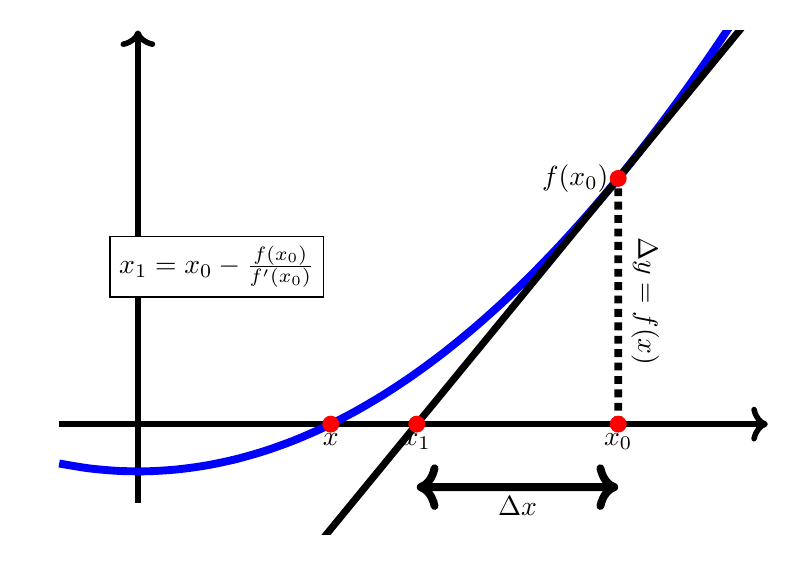
\begin{tikzpicture}[scale=2]

    \newcommand*{\eq}{=}
    \newcommand*{\interceptpos}{3.05}

    % Axis
    \draw[->,thick, line width=.7mm, name path=xaxis] (-.5,0) -- (4,0) coordinate(xlbl);
    \draw[->,thick, line width=.7mm] (0,-.5) -- (0,2.5);

    % fx
    \clip (-.7, -.7) rectangle (4, 2.5);
    \draw[
        -,
        blue,
        domain=-.5:4,
        smooth,
        line width=1mm,
        variable=\x,
        name path=fx
    ] plot ({\x},\x*\x*.2 -.3);

    \filldraw[
        red, 
        name intersections={of=fx and xaxis}
    ] (intersection-1) coordinate(x) circle (.5mm);

    \node at (x)[below] {$x$};

    % Tangent
    \draw[
        -,
        domain=-.5:4,
        smooth,
        line width=.9mm,
        variable=\x,
        black,
        name path=tangent
    ] plot({\x},{2*\interceptpos*.2*(\x - \interceptpos) + (\interceptpos*\interceptpos*.2 -.3)});

    \filldraw[
        red, 
        name intersections={of=tangent and xaxis}
    ] (intersection-1) coordinate(x1) circle (.5mm);

    \node at (x1)[below] {$x_1$};

    % Intercept
    \path[name path=intercept] (\interceptpos, 0) coordinate(x0) -- ++(0, 4);
    \draw[
        dotted, 
        line width=1mm,
        name intersections={of=fx and intercept}
    ] (x0) to [edge label= $\Delta y \eq f(x)$, sloped] (intersection-1) coordinate(v0);

    \filldraw [red] (x0) circle (.5mm);
    \filldraw [red] (v0) circle (.5mm);

    \node at (x0)[below] {$x_0$};
    \node at (v0)[left] {$f(x_0)$};

    \draw[<->, line width=1mm,name path=dx] ($(x1) - (0, .4)$) -- ($(x0) - (0, .4)$) node[pos=0.5](dxlbl){};

    \node at (dxlbl)[below]{$\Delta x$};

    % Formula

    \node[draw, fill=white] at (.5, 1) { $x_1 \eq x_0 - \frac{f(x_0)}{f'(x_0)}$ };


  \end{tikzpicture}
    \caption{
       Graphical representation of the Newton-Raphson method
    }
    \label{fig:pf:nr_graph}
\end{figure}

To make this approach work we need to arrange the power flow \autoref{eq:pf:full_pf_eq}
similar to \autoref{eq:pf:nr_start_point}. We can choose between making $c = I$ or 
$c = S^*$:

\begin{equation}
    \begin{split}
        \sum_{j = 1}^N V_i V_j y_{ij} = S^*_i\\
        \sum_{j = 1}^N V_j y_{ij} = I_i,
    \end{split}
    \label{eq:pf:nr_pf_starting_point}
\end{equation}

thus $f(x)$ becomes:

\begin{equation}
    \begin{split}
        f(x) &= S^*_i(V)\\
        f(x) &= I_i(V),
    \end{split}
    \label{eq:pf:nr:fx_def}
\end{equation}

To formulate Newton-Raphson we also need the derivates $\frac{dS^*_i(V)}{dV}$ or $\frac{dI_i(V)}{dV}$. As $V$ and $S$ are vectors
(one value for each node $i$), the full derivative is a Jacobian:

\begin{align}
    \frac{dS(V)}{dV} = J = 
    \begin{pmatrix}
        \frac{\partial S^*_1}{\partial V_1} & \frac{\partial S^*_1}{\partial V_2} & \dots  & \frac{\partial S^*_1}{\partial V_N}\\
        \frac{\partial S^*_2}{\partial V_1} & \ddots                              &        &                                    \\
        \vdots                              &                                     & \ddots &                                    \\
        \frac{\partial S^*_N}{\partial V_1} &                                     &        & \frac{\partial S^*_N}{\partial V_N}
    \end{pmatrix}.
\end{align}

As these are complex number there are an additional three choices, the derivative can either be taken
with respect to the Cartesian from, Polar form or be left as a complex derivative.\\
\\
All these different choices are mathematically different, but also have an impact
on computational and convergence
performance\autocite{newton_raphson_setup_choices}. Complex formulations
generally perform the worst, whilst Polar and
Cartesian formulations seem to have similar performance.
A current based setup performs slightly better in some 
scenarios\autocite{newton_raphson_setup_choices}.
However, due to the differences being minor, and a 
wider adoption of the polar power formulation, we will use this formulation here.\\

Reformulating eq. \ref{eq:pf:nr_pf_starting_point} in polar yields:

\begin{equation}
    \begin{split}
    P_i = \sum_{j=1}^N |V_i||V_j||y_{ij}| \cos(\theta_{ij} - \delta_i + \delta_j),\\
    Q_i = -\sum_{j=1}^N |V_i||V_j||y_{ij}| \sin(\theta_{ij} - \delta_i + \delta_j).
    \end{split}
    \label{eq:pf:nr_pf_pq}
\end{equation}

To obtain the derivative we can again produce a jacobian:

\begin{equation}
    J =  
    \begin{bmatrix}
        \vec{P}(|\vec{V}|, \ \vec{\delta})\\
        \vec{Q}(|\vec{V}|, \ \vec{\delta})
    \end{bmatrix}
    \begin{pmatrix}
        \frac{\partial}{\partial |\vec{\delta}|} & \frac{\partial}{\partial |\vec{V}|}
    \end{pmatrix}
    =
    \begin{pmatrix}
        \frac{\partial \vec{P}}{\partial \vec{\delta}} & \frac{\partial \vec{P} }{\partial |\vec{V}|}\\
        \frac{\partial \vec{Q}}{\partial \vec{\delta}} & \frac{\partial \vec{Q} }{\partial |\vec{V}|}\\
    \end{pmatrix}
    =
    \begin{pmatrix}
        J_1 & J_2\\
        J_3 & J_4
    \end{pmatrix}.
    \label{eq:pf:nr_pf_jacobi}
\end{equation}

Note that all the values above are vectors, thus each of the entries $J_n$ expand into
their own sub Jacobians.\\

\autoref{eq:pf:nr:fx_def} and \autoref{eq:pf:nr_pf_jacobi} 
can be plugged into \autoref{eq:pf:nr_iteration} as $f(x)$ and $\frac{df}{dx}$
respectively:

\begin{equation}
    V^{(k+1)} = V^{(k)} + (P^{sch} - P^{(k)})J^{-1},
    \label{eq:pf:nr:preliminary}
\end{equation}

where $P^{sch}$ are the power values given as input constraints (used
as $c$) and $P^{(k)}$ the power values
calculated for this iteration.
$V$ and $P$ are row vectors as such:

\begin{equation}
    V = 
    \begin{pmatrix}
        \delta_1\\
        \dots\\
        \delta_N\\
        -\\
        \delta_1\\
        \dots\\
        \delta_N
    \end{pmatrix},
    \quad
    P = 
    \begin{pmatrix}
        P_1\\
        \dots\\
        P_N\\
        -\\
        Q_1\\
        \dots\\
        Q_N
    \end{pmatrix}.
\end{equation}

This also gives us our convergence criteria in the form of:

\begin{equation}
    \begin{split}
        \Delta P &= P^{sch} - P,\\
        |\Delta P| &< \epsilon.
    \end{split}
    \label{eq:pf:nr_pf_convergance}
\end{equation}

\autoref{eq:pf:nr:preliminary} can be re-written with $\Delta P$ as such:

\begin{equation}
    V^{(k+1)} = V^{(k)} + \Delta P \ J^{-1}.
    \label{eq:pf:nr_pf}
\end{equation}

Again \autoref{eq:pf:nr_pf} is applied until
\ref{eq:pf:nr_pf_convergance} is fulfilled.


\section{Creating valid switch states: a graph partitioning problem}

With the atomic islands determined the next step is to generate new swtich states.
A switch state is some combination of open and closed switches,
that results in sets of adjacent nodes that have all switches
between them closed and all switches to other
sets opened.
Further it is a requirement that all the sets
that are being formed to contain exactly
one transformer node. Having more than one transformer is possible, however to
restrict the search space, only configurations with one feeding transformer
will be considered initially.\\
\\
Within the literature this problem is known as graph partitioning, which is a form
of graph covering. 
The specific case needing to be solved here being anchored or 
rooted graph partitioning\autocite{graph_partitioning}. The anchors
or roots being the transformers.\\
\\
Knauer and Ueckerdt\autocite{graph_covering_terminology}
introduce the following terminology for the graph covering problem:
if there is a graph G (called
the host graph) then the set of possible sub-graphs is called a template class.
Elements of the template class are then called template graphs. A configuration 
where each node belongs to at least
one of these templates is called a covering. A quality metric can then be applied to a covering
that grades how well the covering is performing in a certain aspect. For some of these metrics
there exist optimizers that can reliably produce the covering with the best possible result for that
specific quality.\\
Graph partitioning is the same, with one additional constraint, that each node can only belong
to exactly one template. Such a covering is called a partition.\\
Finding switch states is finding graph partitions as each node should only
be contained in exactly one template (be part of one sub-graph) and contain at least
one transformer (one root), making it a rooted partitioning problem.\\
\\
Even for small numbers of nodes there are a huge number of possible partitions
of the grid.
The number of partitions will be referred to as $n_p$.
Just counting how many partitions exist is a non-trivial exercise.
As an upper bound is safe
to assume that

\begin{equation}
    n_p < 2^{n_s} 
    \label{eq:sw_exp:upper_bound1}
\end{equation}

where $n_{s}$ are the number
of switches. This is because each switch can either be opened or closed. However,
a lot of these switch configurations would not result in valid a partition.\\
An approach that could be taken is to generate switch states until a valid
partition is produced. However, this approach is not desirables as
there are a lot more invalid switch states than valid ones. As this
is computationally expensive a better approach is desirable.

\subsection{Random switch states through flooding}
The first method taken was implementing our own graph flooding algorithm that
produces valid partitions. A flooding method is well suited for the problem presented
as it starts at a node and expands out from there to connected nodes. This automatically
ensures that all nodes reached are connected. If the flooding starts at the 
transformer node, it is also ensured that the generated template contains a
transformer. To ensure that the entire graph is covered and that each template contains
exactly one transformer, flooding can be simultaneously started at each transformer.
To generate different switch states the choice of next node to flood to can be
randomized.\\
\\
Algorithmically this can be done by putting each node into its
own set initially.
Next a set of possible next options is formed by considering all neighbours of the
current node. One of them is then randomly chosen to be added to the set.
This process is then repeated until
all nodes have been added to one of the templates. 

\begin{algorithm}[h!]
    \LinesNumbered
    \SetAlgoNoEnd
    \SetAlgoVlined
    \DontPrintSemicolon

    \SetKwFunction{GetRandomTemplates}{getRandomTemplates} % Define the function name
    \SetKwProg{Fn}{Function}{:}{} % Define the keyword and formatting
    \SetKwFunction{GetNextRandom}{getNextRandom}

    \Fn{\GetRandomTemplates{$edgesByNode$, $n$, $startingNodes$}}{

        \tcp{Initialize result templates with each of the initial nodes as the first element of the template}\label{alg:ssexp:random:init_templates}
        $templates \gets \{\}$\;

        \For{$n \in startingNodes$}{
            $templates \gets templates \cup \{n\}$\;
        }

        \tcp{Add nodes to templates until all of them have been visited}\label{alg:ssexp:random:main_loop}
        \While{$|visited| < n$}{

            \tcp{Determine what the next options for expansion for each template are}
            $next \gets \{\}$

            \For{$t \in templates$}{
                $currentNext \gets \{\}$\;
                \For{$node \in t$}{
                    \tcp{For each node in the current template add all neighbouring nodes as a next option, then remove all nodes that have already been visited}
                    $currentNext \gets  (currentNext \cup edgesByNode[node]) \setminus visited$\; 
                }
                $next \gets next \cup \{currentNext\}$\; 
            }

            \tcp{Choose a random template to update and a random node to add to that template out of the possible choices}\label{alg:ssexp:random:get_next}
            $templateChoice, \ nextNodeChoice \gets$ \GetNextRandom{$next$}\;
            
            \tcp{Update the chosen template and the overall visited nodes}
            $templates[templateChoice] \gets templates[templateChoice] \cup nextNodeChoice$\;

            $visited \gets visited \cup nextNodeChoice$\;

        }

        \KwRet $currentSets$\;
    }
    \caption{
        Flooding algorithm to obtain random switch state.
        $edgesByNode$ are the edges of the graph 
        in node representation (see eq. \ref{eq:graph_theory:node_form}),
        $n$ the total number of nodes and $startingNodes$ the node indices to start the flooding at.
    }
    \label{alg:ssexp:random}
\end{algorithm}

\autoref{alg:ssexp:random} outlines how such a random flooding algorithm may look like. The function \texttt{GetNextRandom}
is left as an external call here as changing how that choice is being made will have an effect on the generated template classes.
We have tried two approaches:

\begin{enumerate}
    \item Choose template to expand first, then choose node to expand
    \item Pick an expansion option out of all possible expansion options
\end{enumerate}

These are very different in the probability of which templates gets expanded
and thus the resulting template classes change in their distribution. Equations
\autoref{eq:ssexp:template_probability1} and \autoref{eq:ssexp:template_probability2}
show the probabilities of a template being expanded in any given iteration.

\begin{equation}
    p_{t, 1} = 
    \begin{cases}
        \frac{1}{|\{O_i \in O \ : \ |O_i| > 0\}|} & if \ |O_t| > 0\\
        0 & if \ |O_t| = 0
    \end{cases}
    \label{eq:ssexp:template_probability1}
\end{equation}

\begin{equation}
    p_{t, 2} = \frac{|O_t|}{\sum_{i=0}^{|T|} |O_i|}
    \label{eq:ssexp:template_probability2}
\end{equation}

where $T$ refers to the current set of templates and $O_i$ to the set
of current next expansion options for template $i$. In \autoref{eq:ssexp:template_probability1}
the probability for a template to expand is the same for each template, as long as there
are still expansion options. Meanwhile \autoref{eq:ssexp:template_probability2} implies that
a template is more likely to expand if it has more expansion options.\\
\\

\begin{figure}[H]
    \begin{subfigure}{.5\textwidth}
      \centering
      \includegraphics[width=\linewidth]{img/switchstate_exploring/swiss_suburb/random_switchstate_distribution_tempalte_p.png}
      \caption{}
      \label{fig:ssexp:switchstate_sampels_trafo_p}
    \end{subfigure}%
    \begin{subfigure}{.5\textwidth}
      \centering
      \includegraphics[width=\linewidth]{img/switchstate_exploring/swiss_suburb/random_switchstate_distribution_choice_p.png}
      \caption{}
      \label{fig:ssexp:switchstate_sampels_choice_p}
    \end{subfigure}
    \caption{
        Size of templates generated from \autoref{alg:ssexp:random}
        using \autoref{eq:ssexp:template_probability1} (a) 
        and \autoref{eq:ssexp:template_probability2} (b).
        1000 samples taken. Colours match template colours shown in
        \autoref{fig:data_prep:swiss_suburb_topology_patched}
    }
    \label{fig:ssexp:switchstate_sampels}
\end{figure}

\autoref{fig:ssexp:switchstate_sampels} shows the resulting template size
distributions when applying \autoref{alg:ssexp:random}. As expected, the
template sizes are more evenly distributed when 
using \autoref{eq:ssexp:template_probability1}
then when using \autoref{eq:ssexp:template_probability2}. 
Furthermore, templates generated using
\autoref{eq:ssexp:template_probability2} show a wider
spread of template sizes, whilst almost covering the full range
of sizes generated through \autoref{eq:ssexp:template_probability1}
(The exception being transformers 0, where the template 
never gets as large and transformer 1 where the template never 
gets as small).\\
\\
Due to these results \autoref{eq:ssexp:template_probability2} will
be used to generate switch state samples, as it should cover a wider
range of possible switch states.


% Explain constraints: exactly one trafo per gird, no unconnected nodes 
% Metion literature: anchored graph partitioning

% Expalin algorithm:
% Explain random element

\section{Grid measures}\label{sec:measures}

There are two types of measures that can be applied on a template or on the entire grid 
\begin{enumerate}
  \item A priori measures that result from the grid topology and the parameters
  of the grid components
  \item Measures resulting from running powerflow (or other simulations)
\end{enumerate}

The former are quicker to obtain and are generally good to classify the templates while
the later ones are the most relevant to decide how good a template performs.\\
\\
Ideally a correlation between measures of type one and measures of type two can be
established, as that would make it possible to specifically generate templates
maximizing those quantities.
\\
An added complication arises from the fact that measures that differ per template
might not differ between partitions of the grid. In these cases measures need to be introduced
that assess the difference of this measure between the templates. 

\subsection{A priori measures}

\subsubsection{Atomic island count}

The simplest measure has already been introduced, it is just the number
of atomic island per template: $|T_i|$. The number of atomic
islands in the grid stays constant regardless of switch configuration.
Thus, this measure cannot be used as a comparison between different
partitions.
Further the average template size also doesn't change as: 

\begin{equation}
  \frac{\sum_i^{|T|} |T_i|}{|T|} = \frac{n}{|T|}, \quad \forall T
\end{equation}

To compare the between different partitions the variance, quartiles,
min or max can be used instead.

\subsubsection{Component count}

Component count can be more complicated than atomic island count, depending on how
it is carried out. It could be desirable to exclude dead ends within a template.
These can occur if there is an edge running to a switching cabinet with an open switch. 
In that case it might be desirable to exclude all components in the switching cabinet
and the edge leading to it. If components are excluded depending on the switch state 
counts between partitions may be different and averages hold significance.\\
Of particular interest might
also be counting components of a specific type, like prosumers, cables, etc.

\subsubsection{Geographical extend}

The geographical extent of a grid can be measured in different ways. A simple way is to
measure the distance, $d_{max}$ between the furthest nodes in the grid:

\begin{equation}
  d_{max} = max(\{d_{ij} : i, j < n\})
  \label{eq:measures:geo_extend}
\end{equation}

Similar considerations about excluding components apply.

\subsubsection{Net power}

The net power of a template is the sum over all power produced and consumed:

\begin{equation}
  \sum_{i = 0}^n S_i
\end{equation}

Again this number does not change between partitions.

\subsubsection{Deviation from standard switch state}

There are two main ways to measure this quantify:

\begin{enumerate}
  \item Count how many switch positions are changed
  \item Count the number of atomic islands that have changed template
\end{enumerate}

Option 1 is very well suited as an effort measurement, i.e. how much effort 
it takes the grid operator to switch to that the new state. If $A_x = \{0, 1, ...\}$ 
is the set of switch states where $x$ is a partition and switch positions
are denoted as 1 for closed and 0 for open then

\begin{equation}
\Delta_{s} = |A_a \oplus A_b|
\end{equation}

expresses the number of changed switch positions.\\

Option 2 is well suited to quantify how significant in terms of grid topology 
the change is. If the number of templates stays constant between partitions then:

\begin{equation}
  \Delta_s = \sum_{i=0}^{|T_a|} ||T_{a, i}| - |T_{b, i}||
\end{equation}

\subsubsection{Degree}

The degree of a node is the number of edges connected to it. Using \autoref{eq:graph_theory:node_form}
the degree of a node can be written as:

\begin{equation}
  |\mathfrak{N_i}|
\end{equation}

The average degree
of partitions may be different if open switches are not considered. Similarly, 
if dead ends are disconnected it may change further.

\subsubsection{Density}

The density of a graph is defined as

\begin{equation}
  \frac{2 n_e}{n_n(n_n-1)} 
\end{equation}

It is both useful when applied to the full graph (with open switches removed)
or to individual templates. It can be applied both to the atomic island 
graph or the grid.

\subsubsection{Shortest path length}

The shortest path measures the shortest path between two nodes within a graph.
Particularly useful is the average shortest path length, which considers
the shortest path between any combination of nodes $i$ and $j$. This length can
either be considered as 1 for every edge used, the actual distance in meters or
as the impedance. Unfortunately
the metric is relatively expensive as it scales with the number of nodes squared.\\
An alternative is to take the average distance to a single node. In this case the
transformer should be a good choice.

\subsection{Powerflow based measures}



% - power stats (avg, std, etc)
% - voltage stats
% - line loading stats
% - trafo loading stats
% - Losses

\section{Simulated annealing}

\subsection{Analogy to physical annealing}

Simulated annealing is an optimization method that mimics the
physical process of cooling materials\autocite{simulated_annealing}.
Statistical mechanics teaches us that the probability of a system with
many particles to be in a specific state depends on its energy

\begin{equation}
    p(\{r_i\}) = e^{(-E(\{r_i\})/k_B T)},
\end{equation}

where $k_B$ is Boltzmann's constant, $T$ the temperature, $\{r_i\}$
the set of particle states and $E(\{r_i\})$ the energy of the entire state.
It can be seen that high energy states are more probable at higher temperatures.
However, at lower temperature these higher energy levels become more and more
unlikely. When a material is cooled
that has the ability to configure
into lower energy states it will do so as these lower energy states
are more probable. This process of cooling a material, often with a
specified cooling schedule, to make it settle into a specific type of configuration
is also called annealing, hence the name of the optimization method.\\
The process can be used for optimization by starting with a system at higher
energies and then "cooling" it, hoping for it to settle into a lower energy level.
A key advantage of this method is that it doesn't get stuck in local optima, 
other optimizers. This is because the probability for a higher energy state,
even though it is lower, it is not zero, especially at higher temperatures.

% \subsection{How this relates to switch states}

% To make simulated annealing work we have to model the switch state
% configurations like a statistical system. Firstly 

\subsection{Algorithm}

Simulated annealing as an algorithm works by exploring adjacent
configurations of a system and then assessing the probability of
the system going into the new state based on the energy
of the new and old state. A random draw is then made
utilizing that probability and if it comes out positive, the system
changes into that new state. 

\begin{algorithm}[H]
    
    \SetKwFunction{GetRandomAdjacentState}{getRandomAdjacentState} % Define the function name
    \SetKwFunction{UpdateTemperature}{updateTemperature}
    \SetKwFunction{SimulatedAnnealing}{simulatedAnnealing}
    \SetKwFunction{GetSystemEnergy}{getSystemEnergy}
    \SetKwFunction{P}{p}
    \SetKwFunction{Random}{random}

    \SetKwProg{Fn}{Function}{:}{} % Define the keyword and formatting
    \SetKw{KwContinue}{continue}

    \Fn{\SimulatedAnnealing{$state$, $minTemperature$}}{

        $T \gets 1$\;
        $E_{cur} \gets$ \GetSystemEnergy{$state$}\;

        \While{$T > minTemperature$}{

            $newState \gets$ \GetRandomAdjacentState{$state$}\;
            $E_{new} \gets$ \GetSystemEnergy{$newState$}\;

            $\Delta E \gets E_{cur}-E_{new}$\;

            \If{\P{$\Delta E$, $T$} $>$ \Random{}}{
                $state \gets newState$\;
                $E_{cur} \gets E_{new}$\; 
            }

            $T \gets $ \UpdateTemperature($T$)\;

        }

        \KwRet $state$\;
    }
    \caption{
        Simulated annealing algorithm, where \texttt{p()} is the probability of changing
        states (returns a probability between 0 and 1) and \texttt{random()} produces a
        random number between 0 and 1.
    }
    \label{alg:annealing}
\end{algorithm}

\subsection{Making it work for switch states}

\autoref{alg:annealing} show an implementation of the simulated annealing algorithm.
There are many ways to implement the probability function \texttt{p()}. For this work
a probability closely resembling the Boltzmann probability was chosen:

\begin{equation}
    p_c(\Delta E, T) = \begin{cases}
        1 & \text{if} \ \Delta E \leq 1\\
        e^{(-\gamma \Delta E/ T)} & \text{if} \ \Delta E > 1
    \end{cases} 
\end{equation}

where $\gamma$ is a constant that can be tweaked for best optimization performance.
For the energy of the system the scoring function (\autoref{eq:score}) is used:

\begin{equation}
    E = 1 - s
\end{equation}

Lastly to get a new random adjacent switch state \autoref{alg:ssexp:adjacent}
is used.


\chapter{Results}

\section{Preparing the grid data}

% Explain the atomic island concept
% Inter atomic-island switches
% Explain how this will be the grid we'll be optimizing on
% Explain that we can merge in the atomic islands acting as "leafs" (show comparison graph)grid
% Explain the problem with not connected parts of the grid in the satandard switch case and the solution

To test out different gird configurations some data preparation is required. The following
steps will be showcased utilizing suburban grid data from the aforementioned
Swiss grid operator. The data has been loaded through API calls specified in
\autoref{sec:appendix:api}.\\ For this example
a grid area with the following elements was chosen:

\begin{figure}[H]
    \begin{center}
        \begin{tabular}{ll}
            Grids & 5\\
            Nodes (all types) & 2890\\
            Edges (all types) & 2958\\
            Transformer & 10\\
            Cables & 1995\\
            Prosumers & 600\\
            Switches & 152\\
        \end{tabular}
    \end{center}
    \caption{
        Number of grid elements in the chosen example grid area within a Swiss suburb.
    }
    \label{table:data_prep:swiss_suburban_numbers}
\end{figure}

\subsection{Atomic islands}

To make topological analysis easy and performant atomic islands will be formed.
Figure \ref{fig:data_prep:atomic_islands}
shows some arbitrary grid topology with some nodes and edges. Atomic islands are clusters
of nodes and edges which can not be subdivided by switches further. In the example shown
it is easy to see that two non-divisible clusters can be formed. One containing nodes
1 to 4 and one containing nodes 5 to 8.

\begin{figure}[H]
    \begin{center}
        \includegraphics[width=.6\linewidth]{img/atomic_island.png}
    \end{center}
    \caption{
        Example grid topology with 8 nodes and 9 edges. Switches
        are drawn as a dashed line
    }
    \label{fig:data_prep:atomic_islands}
\end{figure}

To do this algorithmically the edges are considered in edge list
form (\ref{eq:graph_theory:edge_list}). They can then be iterated over.
The nodes are initially put into their own atomic island by themselves.
For each edge that is not a switch, each of the atomic islands on either
side are merged.

\begin{algorithm}[h!]
    \LinesNumbered
    \SetAlgoNoEnd
    \SetAlgoVlined
    \DontPrintSemicolon

    \SetKwFunction{GetConnectedIslands}{getConnectedIslands} % Define the function name
    \SetKwProg{Fn}{Function}{:}{} % Define the keyword and formatting
    \SetKwFunction{GetRandom}{getRandom}

    \SetKw{New}{new}
    \SetKwFunction{Dict}{Dict}

    \Fn{\GetConnectedIslands{$nodes$, $edges$}}{

        \tcp{Initialize all nodes within their own islands and create node to island lookup}
        $I \gets $ \{\}\;
        $islandOfNode \gets $ \New \Dict{}\;

        \ForEach{$node \in nodes$}{
            $I_i \gets   \{ node \}$\;
            $I \gets I \cup \{I_i$\}\;
            $islandOfNode[i] \gets I_i$\;
        }

        \tcp{For any edges merge the islands of the nodes on either end}
        \ForEach{$(i, j) \in edges$}{

            \tcp{Remove the old islands}
            $I \gets I \setminus {islandOfNode[i]}$\;
            $I \gets I \setminus {islandOfNode[j]}$\;

            \tcp{Make a new merged island, update lookup and add that island to the overall list}
            $M \gets islandOfNode[i] \cup islandOfNode[j]$\;
            \ForEach{$k \in M$}{
                $islandOfNode[i] \gets M$\;
            }

            $I \gets I \cup \{M\}$\;
        }
    
        \KwRet $I$\;
    }

    \caption{
        Algorithm to obtain all connected subgraphs (or islands) within a given graph, by providing
        a set of $nodes$ and a set of $edges$ as defined in \autoref{eq:graph_theory:edge_list}
    }
    \label{alg:data_prep:atomic_islands}
\end{algorithm}

\autoref{alg:data_prep:atomic_islands} yields the atomic islands if invoked 
with switches removed from the list of edges:

\begin{equation}
    input = edges \setminus switches
\end{equation}

The same algorithm can be used to generate any other kind of connected subgraphs,
depending on the edges removed.\\
\\
Applying \ref{alg:data_prep:atomic_islands} to the grid area mentioned in table \ref{table:data_prep:swiss_suburban_numbers},
produces an atomic island structure depicted in figure \ref{fig:data_prep:swiss_suburb_with_leafs}.

\begin{figure}[H]
    \begin{center}
        \includegraphics[width=.7\linewidth]{img/switchstate_exploring/swiss_suburb/topology_with_leafs.png}
    \end{center}
    \caption{
        Atomic islands formed out of swiss suburban grid data, laid out in a non-geographical way.
        Atomic islands shown as nodes with 
        ordinary islands in green and islands with transformers as black squares. Connecting switches between the
        atomic islands are shown as edges.
    }
    \label{fig:data_prep:swiss_suburb_with_leafs}
\end{figure}

From figure \ref{fig:data_prep:swiss_suburb_with_leafs} it can be seen, that
there are a lot of leaf nodes present. A leaf node is a node that only has
one connection in the graph structure. I.e. it is a "dead end" within the graph.
For switch state analysis these nodes are not interesting, as the switch leading
up to them can never be open as that would disconnect that leaf node and thus
disconnect the prosumers in that area.\\
This presents us with an opportunity to
reduce the number of nodes and connections needing to be examined further. Reducing the number of
nodes has considerable benefits later on as it speeds up any algorithm
searching through switch state possibilities. It also makes it visually clearer
what the switchable structure of the grid looks like. \\
We can get rid of the leaf nodes by merging them into their neighbouring nodes. 
After merging a leaf into its neighbour the resulting node might now be a leaf. Thus 
the leaf merging algorithm is repeated until there are no leaf nodes left. In the example
case this reduces the number of atomic islands by 801.

\begin{figure}[H]
    \begin{center}
        \includegraphics[width=.8\linewidth]{img/switchstate_exploring/swiss_suburb/topology_sss.png}
    \end{center}
    \caption{
        Atomic islands formed out of Swiss suburban grid data, laid out in a non-geographical way.
        Ordinary atomic islands shown as circles, atomic islands with transformer as squares. Atomic islands connected in the
        standard switch case shown as the same colour. Leaf atomic islands merged.
    }
    \label{fig:data_prep:swiss_suburb_topology}
\end{figure}

The last step in data preparation is to determine the standard switch state (SSS). The standard switch
state is the switch state that the grid is in if there are currently no faults or other abnormal
switching being done. I.e. it is the design switch state that the grid operator currently wants the
grid to be in. It is thus also reasonable to later compare any switch state changes to
the SSS and use it as a benchmark. To determine the SSS
an algorithm like algorithm \ref{alg:data_prep:atomic_islands} can be used again, with the nodes being
the atomic islands and the edges being all switches that are closed in the SSS.\\
\\
Lastly can be the case that there end up being atomic islands that are not connected to any
transformer in the SSS. This can happen if there is another neighbouring grid outwith the selected
geographical bounds or due to data quality issues. To rectify this atomic islands like these will
be merged into the island with the least overall grid load. This is to attempt and balance out
the load on the transformer and make the SSS perform the best it can. In the example
there are two clusters of unconnected atomic islands.
Node 94 (grey) and the orange cluster of nodes.
The result of merging them can be seen in \autoref{fig:data_prep:swiss_suburb_topology_patched}.

\begin{figure}[H]
    \begin{center}
        \includegraphics[width=.8\linewidth]{img/switchstate_exploring/swiss_suburb/topology_sss_patched.png}
    \end{center}
    \caption{
        Atomic islands from \autoref{fig:data_prep:swiss_suburb_topology} with unconnected islands
        connected to their neighbour with the lowest net consumption.
    }
    \label{fig:data_prep:swiss_suburb_topology_patched}
\end{figure}

\subsection{Powerflow}

% Mention how to prepare the data for powerflow

\section{Generating a switch state}

To generate valid switch states we developed two new algorithms. Both make
use of atomic islands.

\subsection{Random switch states through flooding}

The first method taken was implementing our own graph flooding algorithm that
produces valid partitions. A flooding method is well suited for the problem presented
as it starts at a node and expands out from there to connected nodes. This automatically
ensures that all nodes reached are connected. If the flooding starts at the 
transformer node, it is also ensured that the generated template contains a
transformer. To ensure that the entire graph is covered and that each template contains
exactly one transformer, flooding can be simultaneously started at each transformer.
To generate different switch states the choice of next node to flood to can be
randomized.\\
\\
Algorithmically this can be done by putting each node into its
own set initially.
Next a set of possible next options is formed by considering all neighbours of the
current node. One of them is then randomly chosen to be added to the set.
This process is then repeated until
all nodes have been added to one of the templates. 

\begin{algorithm}[h!]


    \SetKwFunction{GetRandomTemplates}{getRandomTemplates} % Define the function name
    \SetKwProg{Fn}{Function}{:}{} % Define the keyword and formatting
    \SetKwFunction{GetNextRandom}{getNextRandom}

    \Fn{\GetRandomTemplates{$edgesByNode$, $n$, $startingNodes$}}{

        \tcp{Initialize result templates with each of the initial nodes as the first element of the template}\label{alg:ssexp:random:init_templates}
        $templates \gets \{\}$\;

        \For{$n \in startingNodes$}{
            $templates \gets templates \cup \{n\}$\;
        }

        \tcp{Add nodes to templates until all of them have been visited}\label{alg:ssexp:random:main_loop}
        \While{$|visited| < n$}{

            \tcp{Determine what the next options for expansion for each template are}
            $next \gets \{\}$

            \For{$t \in templates$}{
                $currentNext \gets \{\}$\;
                \For{$node \in t$}{
                    \tcp{For each node in the current template add all neighbouring nodes as a next option, then remove all nodes that have already been visited}
                    $currentNext \gets  (currentNext \cup edgesByNode[node]) \setminus visited$\; 
                }
                $next \gets next \cup \{currentNext\}$\; 
            }

            \tcp{Choose a random template to update and a random node to add to that template out of the possible choices}\label{alg:ssexp:random:get_next}
            $templateChoice, \ nextNodeChoice \gets$ \GetNextRandom{$next$}\;
            
            \tcp{Update the chosen template and the overall visited nodes}
            $templates[templateChoice] \gets templates[templateChoice] \cup nextNodeChoice$\;

            $visited \gets visited \cup nextNodeChoice$\;

        }

        \KwRet $currentSets$\;
    }
    \caption{
        Flooding algorithm to obtain random switch state.
        $edgesByNode$ are the edges of the graph 
        in node representation (see eq. \ref{eq:graph_theory:node_form}),
        $n$ the total number of nodes and $startingNodes$ the node indices to start the flooding at.
    }
    \label{alg:ssexp:random}
\end{algorithm}

\autoref{alg:ssexp:random} outlines how such a random flooding algorithm may look like. The function \texttt{GetNextRandom}
is left as an external call here as changing how that choice is being made will have an effect on the generated template classes.
We have tried two approaches:

\begin{enumerate}
    \item Choose template to expand first, then choose node to expand
    \item Pick an expansion option out of all possible expansion options
\end{enumerate}

These are very different in the probability of which templates gets expanded
and thus the resulting template classes change in their distribution. Equations
\autoref{eq:ssexp:template_probability1} and \autoref{eq:ssexp:template_probability2}
show the probabilities of a template being expanded in any given iteration.

\begin{equation}
    p_{t, 1} = 
    \begin{cases}
        \frac{1}{|\{O_i \in O \ : \ |O_i| > 0\}|} & if \ |O_t| > 0\\
        0 & if \ |O_t| = 0
    \end{cases}
    \label{eq:ssexp:template_probability1}
\end{equation}

\begin{equation}
    p_{t, 2} = \frac{|O_t|}{\sum_{i=0}^{|T|} |O_i|}
    \label{eq:ssexp:template_probability2}
\end{equation}

where $T$ refers to the current set of templates and $O_i$ to the set
of current next expansion options for template $i$. In \autoref{eq:ssexp:template_probability1}
the probability for a template to expand is the same for each template, as long as there
are still expansion options. Meanwhile \autoref{eq:ssexp:template_probability2} implies that
a template is more likely to expand if it has more expansion options.\\
\\

\begin{figure}[H]
    \begin{subfigure}{.5\textwidth}
      \centering
      \includegraphics[width=\linewidth]{img/switchstate_exploring/swiss_suburb/random_switchstate_distribution_tempalte_p.png}
      \caption{}
      \label{fig:ssexp:switchstate_sampels_trafo_p}
    \end{subfigure}%
    \begin{subfigure}{.5\textwidth}
      \centering
      \includegraphics[width=\linewidth]{img/switchstate_exploring/swiss_suburb/random_switchstate_distribution_choice_p.png}
      \caption{}
      \label{fig:ssexp:switchstate_sampels_choice_p}
    \end{subfigure}
    \caption{
        Size of templates generated from \autoref{alg:ssexp:random}
        using \autoref{eq:ssexp:template_probability1} (a) 
        and \autoref{eq:ssexp:template_probability2} (b).
        Box plots showing the median, the 25\% quartile, the 75\% quartile and outliers used.
        1000 samples taken. Colours match template colours shown in
        \autoref{fig:data_prep:swiss_suburb_topology_patched}
    }
    \label{fig:ssexp:switchstate_sampels}
\end{figure}

\autoref{fig:ssexp:switchstate_sampels} shows the resulting template size
distributions when applying \autoref{alg:ssexp:random}. As expected, the
template sizes are more evenly distributed when 
using \autoref{eq:ssexp:template_probability1}
then when using \autoref{eq:ssexp:template_probability2}. 
Furthermore, templates generated using
\autoref{eq:ssexp:template_probability2} show a wider
spread of template sizes, whilst almost covering the full range
of sizes generated through \autoref{eq:ssexp:template_probability1}
(The exception being transformers 0, where the template 
never gets as large and transformer 1 where the template never 
gets as small).\\
\\
Due to these results \autoref{eq:ssexp:template_probability2} will
be used to generate switch state samples, as it should cover a wider
range of possible switch states.

\subsection{Random adjacent switch state}

Some optimization algorithms work by exploring neighbouring states
of an initial input state. To use these on the atomic island graphs
it is therefore useful to have an algorithm that returns a (random) 
new partition based on the current one. \autoref{alg:ssexp:adjacent}
returns a new partition with the exactly one atomic island changing
templates. 

\begin{algorithm}[H]
    
    \SetKwFunction{GetRandomAdjacentTemplates}{getRandomAdjacentTemplates} % Define the function name
    \SetKwFunction{Clone}{clone} % Define the function name
    \SetKwProg{Fn}{Function}{:}{} % Define the keyword and formatting
    \SetKwFunction{GetRandom}{getRandom}
    \SetKw{KwContinue}{continue}

    \Fn{\GetRandomAdjacentTemplates{$edgesByNode$, $templates$}}{

        \tcp{
            Make a list of all nodes that are on a template boundary
        }
        $possibleFlips \gets \{\}$\;
        \For{$template \in templates$}{
            $currentPossibleFlips \gets \{\}$\;
            \For{$node \in tempalte$}{
                $currentPossibleFlips \gets currentPossibleFlips \cup edgesByNode[node]$\;
            }
            $possibleFlips \gets possibleFlips \cup (currentPossibleFlips \setminus template)$\;
        }

        \While{true}{
            
            \tcp{Clone the templates to leave the old ones untouched}
            $newTemplates \gets$ \Clone{$templates$}\;

            \tcp{Get a random choice of template to enlarge and node to take from another template}
            $templateChoice,\ nodeChoice \gets$ \GetRandom{$possibleFlips$}\;

            \tcp{Update the chosen template with its new node}
            $newTemplates[templateChoice] \gets newTemplates[templateChoice] \cup \{nodeChoice\}$\;
            
            \tcp{Remove the node from its old template}
            \For{$tempalte \in newTemplates$}{
                $template \gets tempalte \setminus \{nodeChoice\}$\; 
            }

            \tcp{
                Check that each template is still valid, i.e. that it still
                has all nodes connected to each other. If not try another random choice
                }
            \For{$template \in newTemplates$}{

                $edges \gets \{\}$\;

                \For{$node \in template$}{
                    $edges \gets edges \cup ((i) \times edgesByNode[node])$
                }

                \If{$|$\GetConnectedIslands{$nodes$, $edges$}$| > 1$}{
                    \KwContinue \;
                }
            }

            
            \KwRet $newTemplates$\;
        }
    }
    \caption{
        Algorithm to get a random new partition with one node changing templates.
        $edgesByNode$ are the edges of the graph 
        in node representation (see eq. \ref{eq:graph_theory:node_form}),
        $teplates$ is an existing partition of a graph.
    }
    \label{alg:ssexp:adjacent}
\end{algorithm}

The method \texttt{getRandom} in \autoref{alg:ssexp:adjacent} works the same
as the \texttt{getNextRandom} in \autoref{alg:ssexp:random}. The probabilities
for a template to expand are similar as presented in equations \ref{eq:ssexp:template_probability1}
and \ref{eq:ssexp:template_probability1}, however $O_i$ instead refers to the number
of nodes connected to a template over an open switch or in other words nodes connected to a 
template belonging to a different template.


\section{Scoring a switch state}\label{sec:score}

We propose the following equation to score a switch state:

\begin{align}
    \begin{split}
        s &= s_{voltage} * w_{voltage}\\
        & + s_{line \ avg} * w_{line \ avg} + s_{line \ max} * w_{line \ max}\\
        & + s_{trafo \ avg} * w_{trafo \ avg} + s_{trafo \ max} * w_{trafo \ max}\\
        & + s_{loss} * w_{loss},
    \end{split}
    \label{eq:score}
\end{align}

where $s_x$ are scores for different operational aspects
and $w_x$ the weights to prioritize or de-prioritize each of these
aspects. The entire equation is normalized to produce values between 0 and 1.\\
As such the weights need to have values between 0 and 1, as well as sum to 1:

\begin{equation}
    w_{voltage} + w_{line \ avg} + w_{line \ max} + w_{trafo \ avg} + w_{trafo \ max} + w_{losses} = 1.
\end{equation}

This equation is introduced by us to unify operating voltage,
line and transformer utilization,
line and transformer limits as well as line losses in a
single score. These 
aspects are the most commonly used ones by grid operators to assess their
grid\autocite{venios}.

\subsection{Voltage score}

We define the voltage score as:

\begin{equation}
    s_{voltage} = clamp(\frac{V_{rated}*(1+\Delta_{V}) - V_{max}
                +       V_{min} - V_{rated}*(1-\Delta_{V})}
                {{V_{rated}*\Delta_{V}}*2}),
                \label{eq:score:voltage}
\end{equation}

where $V_{rated}$ is the rated operating voltage of the grid, $\Delta_V$ the maximum allowed
voltage deviation as a fraction of the rated voltage, $V_{min}$ the minimum voltage  within
the switch state, $V_{max}$ the maximum voltage within the switch state and $clamp()$ being
defined as:

\begin{equation}
    clamp(x) =
    \begin{cases}
        0 & \text{if} \ x < 0\\
        x & \text{if} \ 0 < x < 1\\
        1 & \text{if} \ x > 1
    \end{cases}.
\end{equation}

This score linearly decreases with the minimum and maximum voltages, 
$V_{min}$ and $V_{max}$ deviating further from the rated voltage $V_{rated}$.
The score drops to zero if both $V_{max}$ and $V_{min}$ are outside the
maximum voltage deviation defined through $\Delta_V$.

\subsection{Line utilization score}

The maximum line utilization score is defined as

\begin{equation}
    s_{line \ max} = clamp(\frac{\eta_{line \ max} - max(\{\eta_{ij} : (i, j) \in \mathfrak{E}_{ij}\})}{\eta_{line \ max}})
\end{equation}

average score as

\begin{equation}
    s_{line \ avg} = clamp(\frac{\eta_{line \ avg} - \frac{\sum_{(i, j) \in \mathfrak{E}_{ij}} \eta_{ij}}{|\mathfrak{E}_{ij}|}}{\eta_{line \ avg}}),
\end{equation}

where $\eta_{line \ max}$ and $\eta_{line \ avg}$ are the limits
allowed for the maximum and average currents, before the score drops to 0.
$\eta_{ij}$ is used as defined in \autoref{eq:measures:cable_utilization}.
$\mathfrak{E}_{ij}$ is the set of all cables of the
grid as defined in \autoref{eq:graph_theory:edge_list}
(Important: it is not just the set of edges of one template, but rather of all edges in 
a partition).

\subsection{Transformer utilization score}

The transformer utilization score is defined similarly
to the cable utilization score with

\begin{equation}
    s_{trafo \ max} = clamp(\frac{\eta_{trafo \ max} - max(\{\eta_{t} : 0 < t < |T|\})}{\eta_{trafo \ max}})
\end{equation}

average score as

\begin{equation}
    s_{trafo \ avg} = clamp(\frac{\eta_{trafo \ avg} - \frac{\sum_{t = 0}^{|T|} \eta_t}{|T|}}{\eta_{trafo \ avg}}),
\end{equation}

where $T$ is the set of templates. $\eta_{trafo \ max}$ as well as $\eta_{trafo \ avg}$ 
work similar to the cable limits $\eta_{line \ max}$ and $\eta_{line \ avg}$.

\subsection{Line loss Score}

To calculate a line loss score that is comparable between switch states a suitable
normalization method needs to be employed. The approach taken by us is to use the 
sum over all generated and consumed power as such:

\begin{equation}
    |S|_{total} = \sum_{i=0}^N |P_i| + |Q_i|.
\end{equation}

The rational being, that the more power is generated
or consumed within a grid
the more losses should also occur. 
The absolute value is calculated are component wise
and not as a magnitude as resistive and reactive 
power losses also add up component wise.\\
\\
We define the line loss score as such:

\begin{equation}
    s_{loss} = clamp(\frac{\alpha \sum_{(i, j) \in \mathfrak{E}_{ij}} P_{ij, \ loss} + Q_{ij, \ loss}}{|S|_{total}}),
\end{equation}

where $\alpha$ is a correction term as line losses are usually an order of magnitude
smaller than $|S|_{total}$.

\subsection{Limits and weights used}

\begin{figure}[H]
    \begin{tabular}{l l p{10cm}}
        Limit or weight & Value & Notes\\
        \hline
        $V_{rated}$         & $400V$ & Voltage within the 3-phase low voltage grid\\
        $\Delta_V$          & $0.15$ & $15\%$ voltage deviation is often used as an acceptable limit by grid operators\autocite{venios}\\
        $\eta_{line \ avg}$ & $1$    & \\
        $\eta_{line \ max}$ & $2.5$  & Rated current is not maximum allowed current, as such higher currents may occur\\
        $\eta_{trafo \ avg}$& $1$    & \\
        $\eta_{trafo \ max}$& $1.5$  & Rated power is not maximum allowed power, as such higher currents may occur\\
        $\alpha$            & $40$   & Determined through trial and error\\
        $w_{voltage}$       & $1/4$  & All 4 score categories set to contribute equally\\
        $w_{line \ avg}$    & $1/8$  & All 4 score categories set to contribute equally, there are 2 line utilization measures\\
        $w_{line \ max}$    & $1/8$  & All 4 score categories set to contribute equally, there are 2 line utilization measures\\
        $w_{trafo\ avg}$    & $1/8$  & All 4 score categories set to contribute equally, there are 2 transformer utilization measures\\
        $w_{trafo\ max}$    & $1/8$  & All 4 score categories set to contribute equally, there are 2 transformer utilization measures\\
        $w_{loss}$          & $1/4$  & All 4 score categories set to contribute equally
    \end{tabular}
    \caption{Values used for the score function \autoref{eq:score}}
    \label{table:score:values}
\end{figure}

As mentioned all weights and limits are chosen such that they are meaningful to grid operators
and can be tweaked by them as needed. For all switch state scores within this work the values
in \autoref{table:score:values} have been used.


\section{Powerflow implementations}\label{sec:pf:impl}

\subsection{Implementations}

All powerflow solver code can be found in 
\texttt{lib/powerflow.py}, \texttt{lib/fastpf/powerflow.h}
\\ and
\texttt{lib/fastpf/powerflow.c}\\

The methods \texttt{solve\_powerflow\_gauss\_seidel()}
and \texttt{solve\_powerflow\_newton\_raphson()}
use python and numpy only and closely follow the mathematical formulations layed out above.\\

For the Gauss-Seidel method it is worth mentioning, that the Voltage result for each
node (\ref{eq:pf:gs_pf}) is immediately used to update the voltage vector. I.e. when $V_i^{(k+1)}$
is calculated the voltages $V_{j}^{(k+1)}$ where $j<i$ are already available and being used instead of
the old values $V_{j}^{(k)}$.\\

These methods where used as a baseline to access their performance. To identify where the biggest
speed-ups in performance could be gained timings where recorded for each of stages in the algorithm.
For a run of the python only Newton-Raphson timings to calculate the simbench grid shown in figure
\ref{fig:vep:simbench_node_types} are listed below:

\vspace{.5cm}

\begin{figure}[H]
    \begin{center}
        \begin{tabular}{ll}
            \textbf{Method section} & \textbf{Time (ms)}\\
            \hline
            Prepare matrices and vectors & 0.108\\
            Fill jacobian with zeros &  0.050\\
            Fill jacobian with values & 296.843\\
            Calculate Deltas &      0.067\\
            Invert Jacobian &      1.099\\
            Update voltage vector & 0.235\\
            \hline
            \textbf{Total} & \textbf{298.487}
        \end{tabular}
    \end{center}
\caption{Timings taken for different parts of the \texttt{solve\_powerflow\_newton\_raphson()} method}
\end{figure}
    
From this table it can immediately be seen, that the most important part
of the algorithm to optimize is filling the Jacobian with values. Thus, this
part was implemented in c using python c bindings to directly fill a numpy
matrix passed with values. This has the major advantage that only the most performance
critical code has to be implemented in c whilst everything else can be kept in python
for easy and quick development. Additionally, passing an existing matrix from python
means no additional memory allocations have to be done in c which is both good for performance 
and memory safety.\\
Taking the same timing for the c enhanced Newton-Raphson implementation yields the following:

\begin{figure}[H]
    \begin{center}
        \begin{tabular}{ll}
            \textbf{Method section} & \textbf{Time (ms)}\\
            \hline
            Prepare matrices and vectors & 0.232\\
            Fill jacobian with zeros &  0.051\\
            Fill jacobian with values & 0.436\\
            Calculate Deltas &      0.032\\
            Invert Jacobian &      1.493\\
            Update voltage vector & 0.016\\
            Finalize & 0.016\\
            \hline
            \textbf{Total} & \textbf{2.276}
        \end{tabular}
    \end{center}
\caption{Timings taken for different parts of the \texttt{fast\_newton\_raphson()} method}
\end{figure}

Using the new c method yields a considerable speed-up by more than ten times.\\

To unlock a further speed gain the matrices in use need to be examined closely. A normal admittance matrix has 
an entry for every possible combination of nodes $i$ and $j$, this means it has size $N^2$. However, if there is
no cable betewen $i$ and $j$ this entry is zero. As a lot of these cables do not exist a lot of the entries are zero
and the admittance matrix is sparse.
As can be seen from equation \ref{eq:pf:nr_pf_jacobi} as well as \ref{eq:pf:nr_pf_p} and \ref{eq:pf:nr_pf_q} the entries
in the Jacobian are also zero if a given entry $y_{ij}$ is zero in the admittance matrix.\\
Just iterating over these zero entries or doing multiplications of zero values wastes considerable processor time. On top
the large matrices take up a lot of memory. This problem can be solved by specifically using
a sparse matrix library like \textit{scipy.sparse}\autocite{2020SciPy-NMeth}. The library offers
data types that only store non-zero elements within the matrix as well as solvers that can operate
efficiently on these types.\\
Using the sparse library as well as implementing c code that operates on this matrix type a
further performance gain is possible:

\begin{figure}[H]
    \begin{center}
        \begin{tabular}{ll}
            \textbf{Method section} & \textbf{Time (ms)}\\
            \hline
            Prepare matrices and vectors & 0.075\\
            Fill power vec. with zeros &  0.007\\
            Fill jacobian with values & 0.179\\
            Calculate Deltas &      0.024\\
            Invert Jacobian &      0.452\\
            Update voltage vector & 0.015\\
            Finalize & 0.013\\
            \hline
            \textbf{Total} & \textbf{0.765}
        \end{tabular}
    \end{center}
\caption{Timings taken for different parts of the \texttt{fast\_newton\_raphson\_sparse()} method}
\end{figure}

\subsection{Validation}

\subsubsection{Simple 3 node grid}

\begin{figure}[H]
    \centering
    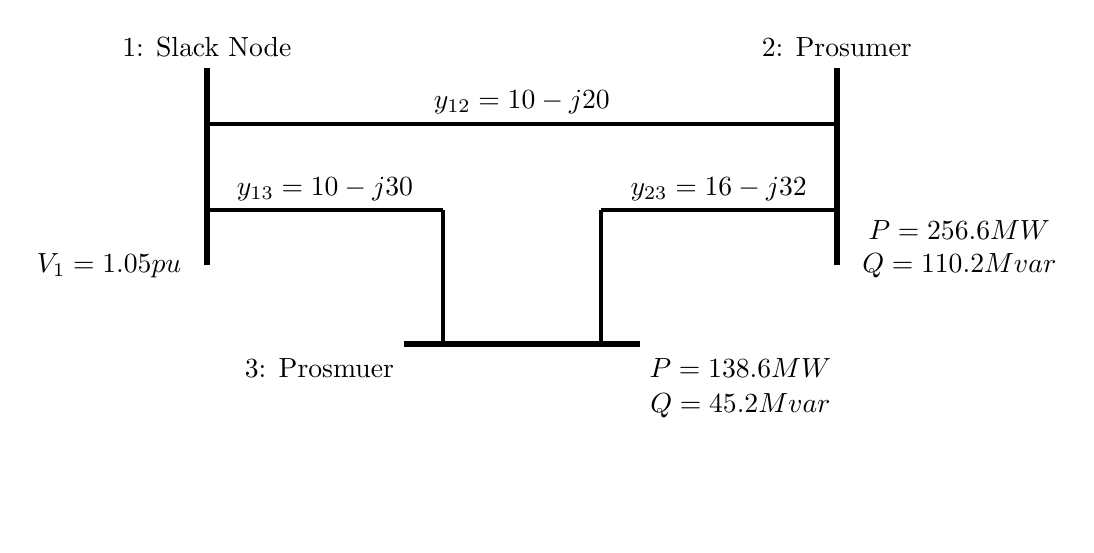
\begin{tikzpicture}[scale=1]


    % Slack
    \draw[line width=.8mm] (-4, -1) coordinate(s1) -- ++(0, 2.5) coordinate(e1) node(slack)[above]{1: Slack Node};
    \node (voltage_label) at ($(s1) - (.2, 0)$)[left] {$V_1 = 1.05 pu$};

    % Load 1
    \draw[line width=.8mm] (4, -1) coordinate(s2) -- ++(0, 2.5) coordinate(e2) node(slack)[above]{2: Prosumer};
    \node (q_label1) at ($(s2) + (.2, 0)$)[left][right] {$Q = 110.2Mvar$};
    \node (p_label1) at ([yshift=2mm]q_label1)[above] {$P = 256.6MW$};

    % Load 2
    \draw[line width=.8mm, name path=l2] (-1.5, -2) coordinate(s3) -- ++(3, 0) coordinate(e3);
    \node(slack) at ($(s3) - (0, .3)$)[left]{3: Prosmuer};
    \node(p_label2) at ($(e3) - (0, .3)$)[right]{$P = 138.6MW$};
    \node(q_label2) at ([yshift=-2mm]p_label2)[below]{$Q = 45.2 Mvar$};

    % Lines
    \draw[line width=.5mm] ($(e1) - (0, .7)$) -- ($(e2) - (0, .7)$) node[pos=.5](l1_midpoint){};
    \node(line_lbl_1) at (l1_midpoint)[above]{$y_{12} = 10-j20$};

    \draw[line width=.5mm] ($(s1) + (0, .7)$) -- ++(3, 0) coordinate(l2_end) node[pos=.5](l2_midpoint){};
    \node(line_lbl_2) at (l2_midpoint)[above]{$y_{13} = 10-j30$};

    \path[name path=intercept] (l2_end) -- ++(0, -4);
    \draw[
        line width=.5mm,
        name intersections={of=intercept and l2}
    ] (l2_end) to (intersection-1);

    \draw[line width=.5mm] ($(s2) + (0, .7)$) -- ++(-3, 0) coordinate(l3_end) node[pos=.5](l3_midpoint){};
    \node(line_lbl_3) at (l3_midpoint)[above]{$y_{23} = 16-j32$};

    \path[name path=intercept2] (l3_end) -- ++(0, -4);
    \draw[
        line width=.5mm,
        name intersections={of=intercept2 and l2}
    ] (l3_end) to (intersection-1);

  \end{tikzpicture}
    \caption{
        A simple 3 node system taken from \textit{Power System Analysis}\autocite{power_system_analysis}.
        Admittances $y_{ij}$ are in $pu$ (power unit) on a 100-MVA base.
        $P$ and $Q$ of prosumers are positive for consumption and negative for production.
    }
    \label{fig:pf:3_node_system}
\end{figure}


Fast powerflow is good, but no use if it is not correct. For validation
the solvers are compared against the system shown in figure \ref{fig:pf:3_node_system} and results
provided in \textit{Power System Analysis}\autocite{power_system_analysis}.

\begin{figure}[H]
    \begin{center}
        \begin{tabular}{m{3cm} | m{2.5cm} m{2.5cm} m{2.5cm} m{2.5cm}}
            Method & Slack real Power $P_1$ (MW) & Slack reactive Power $Q_1$ (Mvar) & Node 2 Voltage $V_2$ ($pu$) & Node 3 Voltage $V_2$ ($pu$)\\
            \hline
            Gauss-Seidel in \textit{Power System Analysis}\autocite{power_system_analysis} & $409.5$ & $189$ & $0.9800 - j0.0600$ & $1.0000 - j0.0500$\\
            \hline
            Own Gauss-Seidel implementation & 409.4 & 188.9 & $0.9800-j0.0600$ & $1.0000 - j0.0500$ \\
            \hline
            Own Newton-Raphson implementation (basic) & 409.5 & 189 & $0.9800-j0.0600$ & $1.0000 - j0.0500$ \\
        \end{tabular}
    \end{center}
    \caption{Results obtained through different methods for the grid shown in figure \ref{fig:pf:3_node_system}}
\end{figure}

The table above shows that the results obtained with our own Gauss-Seidel and Newton-Raphson
implementations agree with each other and with the values calculated in \textit{Power System Analysis}\autocite{power_system_analysis}. The accelerated
Newton-Raphson methods have also been compared with the values shown above, they are exactly equal to the values 
for the basic Newton-Raphson implementation

\subsubsection{Pandapower}

A second validation was carried out against the widely used open source package
\textit{panadapower}\autocite{pandapower2018}. The \textit{Simbench} grid
introduced in \autoref{fig:vep:simbench_node_types} was used here. Values
produced by \textit{panadapower} and our implementation agree exactly.

\subsection{Performance}


\begin{figure}[H]
    \centering
    \includegraphics[width=.65\linewidth]{img/benchmark/pandapower_avg.png}
    \caption{
        Iteration time of \textit{pandapower}\autocite{pandapower2018} Newton-Raphson and our implementation of
        Newton-Raphson vs. grid size. 20 samples taken for every grid size. Simbench
        grid (\autoref{fig:vep:simbench_node_types}) used and shrunk by cutting
        away outer nodes. Admittance matrix creation and result power vector creation 
        is included in the timings for our method as \textit{pandapower} is also calculating
        these values
    }
    \label{fig:pf:benchmark}
\end{figure}

\autoref{fig:pf:benchmark} shows the performance difference between our method and \textit{pandapower}.
Our method is up to an order of magnitude faster than \textit{pandapower} and has better timing
consistency. Egor Grishin et. al. show that \textit{pandapower} is among the faster power flow
implementations available in python\autocite{newton_raphson_python}. Our method should therefore
be as fast or faster than the fastest available python Newton-Raphson implementations.\\
\\
That this is the case will partially be due to the vastly reduced feature set of our method
(it just calculates the voltage vector based on the admittance matrix). However, to write
something like a switch state optimizer, this is all that is needed, and the additional
performance makes a big difference in how many switch states can be assessed in a given time.


\section{Randomly generated switch states}



\begin{figure}[H]
    \begin{subfigure}{.33\textwidth}
      \centering
      \includegraphics[width=\linewidth]{img/switchstate_exploring/swiss_suburb/histograms/avg_cable_util.png}
      \caption{}
      \label{fig:result:suburban:histograms:avg_cable}
    \end{subfigure}%
    \begin{subfigure}{.33\textwidth}
      \centering
      \includegraphics[width=\linewidth]{img/switchstate_exploring/swiss_suburb/histograms/max_cable_util.png}
      \caption{}
      \label{fig:result:suburban:histograms:max_cable}
    \end{subfigure}
    \begin{subfigure}{.33\textwidth}
        \centering
        \includegraphics[width=\linewidth]{img/switchstate_exploring/swiss_suburb/histograms/avg_trafo_util.png}
        \caption{}
        \label{fig:result:suburban:histograms:avg_trafo}
      \end{subfigure}\\
      \begin{subfigure}{.33\textwidth}
        \centering
        \includegraphics[width=\linewidth]{img/switchstate_exploring/swiss_suburb/histograms/max_trafo_util.png}
        \caption{}
        \label{fig:result:suburban:histograms:max_trafo}
      \end{subfigure}%
      \begin{subfigure}{.33\textwidth}
        \centering
        \includegraphics[width=\linewidth]{img/switchstate_exploring/swiss_suburb/histograms/line_loss.png}
        \caption{}
        \label{fig:result:suburban:histograms:line_loss}
      \end{subfigure}%
      \begin{subfigure}{.33\textwidth}
        \centering
        \includegraphics[width=\linewidth]{img/switchstate_exploring/swiss_suburb/histograms/line_loss_relative.png}
        \caption{}
        \label{fig:result:suburban:histograms:line_loss_rel}
      \end{subfigure}\\
      \begin{subfigure}{.33\textwidth}
        \centering
        \includegraphics[width=\linewidth]{img/switchstate_exploring/swiss_suburb/histograms/min_voltage.png}
        \caption{}
        \label{fig:result:suburban:histograms:min_voltage}
      \end{subfigure}%
      \begin{subfigure}{.33\textwidth}
        \centering
        \includegraphics[width=\linewidth]{img/switchstate_exploring/swiss_suburb/histograms/score.png}
        \caption{}
        \label{fig:result:suburban:histograms:score}
      \end{subfigure}
    \caption{Power produced/consumed by a household (a) and a solar panel (b) within a SimBench grid at different times of day and at different times of year. Data is generated by a standard laod profile model within VEP and obtained over API\autocite{venios}}
    \label{fig:result:suburban:histograms}
\end{figure}

\section{Correlation of structural/topological and operational measures}

\begin{figure}[H]
    \begin{center}
        \includegraphics[width=\linewidth]{img/switchstate_exploring/swiss_suburb/correleation.png}
    \end{center}
    \caption{
        Correlation plots between topological/structural grid measures and 
        operational grid measures. Grid area as introduced In
        \autoref{fig:data_prep:swiss_suburb_topology_patched}.
        Data points in red are the SSS and in green the best random switch state.
        Refer to \autoref{sec:measures} for more
        information on the individual measures.
    }
    \label{fig:correlation}
\end{figure}

\autoref{fig:correlation} shows structural/topological grid
measures (\autoref{sec:topo_and_struct_measures}) vs. 
operational grid measures (\autoref{sec:operational_measures}). 
Some measures show almost linear relationships, like
the template size standard deviation (\autoref{sec:island_count}) vs.
the average transformer utilization. Other relations seem
to be fully random such as average geographical extend (\autoref{eq:measures:geo_extend})
vs. average cable utilization. Most relations lie in-between, there is
clearly some correlation, however it does not seem like it could
be captured through any simple formula.\\
\\
By far the most interesting relation that can be seen is 
average steps to the next transformer (\autoref{sec:shortest_path})
vs. score. The data seems to
suggest that the highest scores only exist at low average
step counts. It seems like a direct optimization for 
the average steps to the transformer could be performed in this grid
area instead for optimizing for score. As calculating the steps
is computationally cheaper than calculating the score this would
potentially allow for very fast optimization.\\
\\
Unfortunately these relations seem not to hold across grid areas
(compare \autoref{fig:appendix:suburb2:correleation} and \autoref{fig:appendix:suburb2:correleation}).
It seems like that the correlation between these measures is highly
dependent on the specific grid area examined. This means that
no universal optimizer optimizing for the presented
structural/topological measures can be developed.\\
\\
Further examination is certainly required, to determine if there
are any wider correlations holding across grid areas.



\section{Simulated annealing}

To make simulated annealing work for switch states
we have to supply the missing functions and values
in \autoref{alg:annealing}.\\
There are many ways to implement the probability function \texttt{p()}. For this work
a probability closely resembling the Boltzmann probability was chosen:

\begin{equation}
    p_c(\Delta E, T) = \begin{cases}
        1 & \text{if} \ \Delta E \leq 1\\
        e^{(-\gamma \Delta E/ T)} & \text{if} \ \Delta E > 1
    \end{cases} 
\end{equation}

where $\gamma$ is a constant that can be tweaked for best optimization performance.
For the energy of the system the scoring function (\autoref{eq:score}) is used:

\begin{equation}
    E = 1 - s
\end{equation}

A new random adjacent switch state is generated with \autoref{alg:ssexp:adjacent}.

\subsection{Annealing results}

\begin{figure}[H]
    \centering
    \begin{tabular}{lrrr}
        \toprule
        & SSS & Best random & Best annealed\\
        \midrule
        Score (x100) & 63.1 & 72.5 & 73.7 \\
        Min. Voltage (V) & 369.5 & 389.5 & 389.5 \\
        Max. cable utilization (\%) & 124.7 & 93.6 & 93.6 \\
        Avg. cable utilization (\%) & 17.0 & 16.6 & 16.2 \\
        Max. transformer utilization (\%) & 66.2 & 62.9 & 54.4 \\
        Avg. transformer utilization (\%) & 35.8 & 33.3 & 33.9 \\
        Toal line losses (kW) & 51.6 & 39.0 & 36.5 \\
        \bottomrule
    \end{tabular}
    \caption{
        Table showing the highest scores obtained through simulated annealing
        and random switch state generation vs. the standard switch sate. Refer
        to \autoref{sec:measures} and to \autoref{sec:score} for an explanation
        of the measures used.
    }
    \label{table:annealing:compare}
\end{figure}

The values for the simulated annealing section where obtained using
the "Suburb 2" area. More information about this grid area can be
found in  \autoref{sec:appendix:suburb2}. A comparison
between the SSS and the optimized switch states
can be found in \autoref{table:annealing:compare}. 

\begin{figure}[H]
    \begin{subfigure}{.5\textwidth}
      \centering
      \includegraphics[width=\linewidth]{img/switchstate_exploring/suburb2/annealing_sampling/alhpa.png}
      \caption{}
    \end{subfigure}%
    \begin{subfigure}{.5\textwidth}
      \centering
      \includegraphics[width=\linewidth]{img/switchstate_exploring/suburb2/annealing_sampling/beta.png}
      \caption{}
    \end{subfigure}\\
    \begin{subfigure}{.5\textwidth}
        \centering
        \includegraphics[width=\linewidth]{img/switchstate_exploring/suburb2/annealing_sampling/p_multi.png}
        \caption{}
    \end{subfigure}%
    \begin{subfigure}{.5\textwidth}
        \centering
        \includegraphics[width=\linewidth]{img/switchstate_exploring/suburb2/annealing_sampling/starting_score.png}
        \caption{}
    \end{subfigure}
    \caption{
        Simulated annealing applied to the "Suburb 2" grid area (\autoref{sec:appendix:suburb2}).
        Plotting score $s$ reached vs. varying values of $\alpha$ (a), $\gamma$ (b), $p_{multi}$ (c) and
        the score of the random switch state configuration that was used as the initial state (d).
        Box plots showing the median, the 25\% quartile, the 75\% quartile and outliers used for (a), (b) and (c).
        6 samples taken for each configuration in (a), (b) and (c). (d) shows all samples of all configurations.
        Initial random switch states where obtained through \autoref{alg:ssexp:random}.
        The standard values where $\alpha = 0.99$, $\beta = 1000$ and $p_{multi} = 0.33$
        when other parameters where examined.
    }
    \label{fig:annealing:parameters}
\end{figure}

\autoref{fig:annealing:parameters} shows the score reached by the annealed grid area
with varying parameterizations and starting switch states. The most surprising result
is that the best score of around $s = 0.75$ can be reached no matter what
the starting switch state is and no matter the parameters chosen. This
seems to suggest that there is an absolute ceiling for the best score that
can be achieved through annealing at that value. This could either be due
to a fundamental limit of the method itself or it could be that this switch
state is actually the optimal switch state and that no better switch state
exists at all. The later conclusion might be supported by the fact that the
four best switch states found are all the same (see \autoref{fig:annealing:topologies})\\
\\
We also cautiously conclude that values of around $\gamma = 400$ and $p_{multi} > 0.8$
make it most probable to reach the maximum score. However, a larger sample size
will be required to determine this. Running the annealing algorithm takes some time
as can be seen in \autoref{fig:annealing:over_time}. Multiple samples have to be taken as
not all trials yield a similar score. 

\begin{figure}[H]
    \begin{subfigure}{.5\textwidth}
      \centering
      \includegraphics[width=\linewidth]{img/switchstate_exploring/suburb2/annealing_sampling/best_overall.png}
      \caption{
       }
      \label{fig:annealing:topologies}
    \end{subfigure}%
    \begin{subfigure}{.5\textwidth}
      \centering
      \includegraphics[width=\linewidth]{img/switchstate_exploring/suburb2/annealing_sampling/over_time.png}
      \caption{
      }
      \label{fig:annealing:over_time}
    \end{subfigure}
    \caption{
        (a) The 4 highest scoring switch states reached after annealing. Best overall
        scores and switch states from runs shown in \autoref{fig:annealing:parameters} taken.
        Layout produced with
        Kamada-Kawai layout algorithm\autocite{kamada_kawai}.\\
        (b) Scores reached through simulated annealing after a running the
        algorithm for some time. 6 samples. $\gamma = 400$, $\alpha = 0.99$ and $p_{multi} = 0.33$
    }
\end{figure}


    


% Show distributions of pre-powerflow data (perhaps per grid)

\section{Changing laod data over time}

\begin{figure}[H]
    \begin{subfigure}{.5\textwidth}
      \centering
      \includegraphics[width=\linewidth]{img/switchstate_exploring/suburb2/compare_over_time.png}
      \caption{}
      \label{fig:time:suburb2:sss_vs_optimized}
    \end{subfigure}%
    \begin{subfigure}{.5\textwidth}
        \centering
        \includegraphics[width=\linewidth]{img/switchstate_exploring/urban2/compare_over_time.png}
        \caption{}
        \label{fig:time:urban2:sss_vs_optimized}
    \end{subfigure}
    \caption{}
    \label{fig:time:sss_vs_optimized}
\end{figure}
\begin{figure}[H]
    \begin{subfigure}{.5\textwidth}
        \centering
        \includegraphics[width=\linewidth]{img/switchstate_exploring/suburb2/switchstates_over_time.png}
        \caption{}
        \label{fig:time:suburb2:best_at_different_times}
    \end{subfigure}%
    \begin{subfigure}{.5\textwidth}
        \centering
        \includegraphics[width=\linewidth]{img/switchstate_exploring/urban2/switchstates_over_time.png}
        \caption{}
        \label{fig:time:urban2:best_at_different_times}
    \end{subfigure}
    \caption{}
    \label{fig:time:best_at_different_times}
\end{figure}

\chapter{Conclusion}

% Score works to balance grid measurs
% There are better switch state !!!!
% We can reliably find them
% Pf works and is the the better perforamnce enables this analysis
% 

\chapter{Appendix}

\section{Venios API}\label{sec:appendix:api}

Data elements in VEP are identified by their \texttt{ForeignKey} (abbrv. to \texttt{FK}). This is a unique key which
uniquely identifies the element and is sufficient to retrieve it. Data retrieved from the API might
be a combination of many data elements and might therefore not have a single \texttt{ForeignKey}, however
it might mention other elements by their \texttt{ForeignKey} so that they can be retrieved.

\subsection{API methods}

\begin{tabular}{ l  p{12cm}} 
    \hline
    \multicolumn{2}{c}{\textbf{Voltage Groups}}\\
    \hline
    Method Name     & \texttt{GetAllVoltageGroups} \\
    Input           & -\\
    Output          & \texttt{list of VoltageLevel} \\
    Description     & Returns all voltage levels available in the current VEP instance. A voltage level is a level within the grid, normal households are usually connected to the LV (low voltage) voltage level at 400V\\
\end{tabular}

\vspace{.5cm}

\begin{tabular}{ l  p{12cm}} 
    \hline
    \multicolumn{2}{c}{\textbf{Grids in Geographical Boundary}}\\
    \hline
    Method Name     & \texttt{LoadGridsInGeoBounds} \\
    Input           & \texttt{VoltageLevel, GeoBounds}\\
    Output          & \texttt{list of GridFK}\\
    Description     & Returns foreign keys to grids within a geographical boundary and voltage level. A "grid" in vep is an administrative set of grid components usually connected to one transformer\\
\end{tabular}

\vspace{.5cm}

\begin{tabular}{ l  p{12cm}} 
    \hline
    \multicolumn{2}{c}{\textbf{Conducting Topology}}\\
    \hline
    Method Name     & \texttt{LoadManyConductingTopologies} \\
    Input           & \texttt{list of GridFK}\\
    Output          & \texttt{GridTopology} \\
    Description     & Returns the conducting topology of a grid, these are its cables, nodes and transformers\\
\end{tabular}

\vspace{.5cm}

\begin{tabular}{ l  p{12cm}} 
    \hline
    \multicolumn{2}{c}{\textbf{Get Many}}\\
    \hline
    Method Name     & \texttt{GetMany} \\
    Input           & \texttt{list of FK}\\
    Output          & Raw VEP data element \\
    Description     & Used to retrieve a list of VEP data elements of any data type. Used here to retrieve transformer and cable specifications\\
\end{tabular}

\vspace{.5cm}

\begin{tabular}{ l  p{12cm}} 
    \hline
    \multicolumn{2}{c}{\textbf{Load Profiles}}\\
    \hline
    Method Name     & \texttt{GetLoadProfiles} \\
    Input           & \texttt{list of ProsumerFK, start datetime, end datetime, resolution, model prefrences}\\
    Output          & list of complex Power values \\
    Description     & Returns a load values over time from a start datetime to an end datetime with the resolution specified. If multiple models to generate load profiles are available a preferred model can be specified \\
\end{tabular}

\subsection{Complex data types}

Below is a description of the relevant complex data types retrieved from VEP. This is an incomplete
description only showing relevant data fields.

\vspace{.5cm}

\begin{tabular}{ l p{3cm} l p{8cm}} 
    \hline
    \multicolumn{4}{c}{\texttt{VoltageLevel}}\\
    \hline
    \textbf{Field Name} & \textbf{Data Type}       & \textbf{Unit} & \textbf{Description} \\
    \hline
    LowerLimit          & \texttt{double}          & $V$           & Lower voltage limit of this voltage level\\
    UpperLimit          & \texttt{double}          & $V$           & Upper voltage limit of this voltage level\\
    ForeignKey          & \texttt{ForeignKey}      &               & \texttt{ForeignKey} of this voltage level
\end{tabular}

\vspace{.5cm}

\begin{tabular}{ l p{3cm} l p{8cm}} 
    \hline
    \multicolumn{4}{c}{\texttt{GridTopology}}\\
    \hline
    \textbf{Field Name} & \textbf{Data Type}              & \textbf{Unit} & \textbf{Description} \\
    \hline
    GridFK              & \texttt{ForeignKey}                       &               & \texttt{ForeignKey} of the grid\\
    Transformer         & \texttt{list of GridElement}    &         & All transformers of the grid\\
    Edges               & \texttt{list of GridElement}    &         & All edges of the grid (without transformers which are also an edge in VEP)\\
    Nodes               & \texttt{list of GridElement}    &         & All nodes of the grid \\
\end{tabular}

\vspace{.5cm}

\begin{tabular}{ l p{3cm} l p{8cm}} 
    \hline
    \multicolumn{4}{c}{\texttt{GridElement}}\\
    \hline
    \textbf{Field Name} & \textbf{Data Type}            & \textbf{Unit} & \textbf{Description} \\
    \hline
    PrimaryKey          & \texttt{ForeignKey}           &               & The primary key of the corresponding VEP data element\\
    Name                & \texttt{string}               &               & Name of the element given by the grid operator\\
    \hline
    \multicolumn{4}{c}{\textbf{if edge}}\\
    \hline
    NodeA               & \texttt{ForeignKey}           &               & Node connected on side A\\
    NodeB               & \texttt{ForeignKey}           &               & Node connected on side B\\
    \hline
    \multicolumn{4}{c}{\textbf{if Cable or Transformer}}\\
    \hline
    Specs               & \texttt{list of SpecificationFK}             &               & \texttt{ForeignKey} to the specification specifying physical parameters of the transformer or cable\\
    \hline
    \multicolumn{4}{c}{\textbf{if Cable}}\\
    \hline
    Length              & \texttt{double}              &  $m$          & Length of the cable\\
    \hline
    \multicolumn{4}{c}{\textbf{if Switch}}\\
    \hline
    DefaultSwitchState  & \texttt{boolean}             &               & True if the switch is closed in the default configuration\\
    CurrentSwitchState  & \texttt{boolean}             &               & True if the switch is currently closed\\
\end{tabular}

\vspace{.5cm}

\begin{tabular}{ l p{3cm} l p{8cm}} 
    \hline
    \multicolumn{4}{c}{\texttt{Cable Specification}}\\
    \hline
    \textbf{Field Name} & \textbf{Data Type}        & \textbf{Unit} & \textbf{Description} \\
    \hline
    NominalCurrent      & \texttt{double}           & $A$           & Max. operating current in amps\\              
    Resistance20        & \texttt{double}           & $\Omega/m$    & Resistance at $20C^\circ$\\  
    Reactance           & \texttt{double}           & $\Omega/m$    & Reactance\\              
\end{tabular}

\begin{tabular}{ l p{3cm} l p{8cm}} 
    \hline
    \multicolumn{4}{c}{\texttt{Transformer Specification}}\\
    \hline
    \textbf{Field Name} & \textbf{Data Type}        & \textbf{Unit} & \textbf{Description} \\
    \hline
    RatedPower          & \texttt{double}           & $VA$          & Max. operating power\\              
   \end{tabular}

\vspace{1cm}


\section{"Suburb 2" grid area}\label{sec:appendix:suburb2}

\begin{figure}[H]
  \begin{center}
      \includegraphics[width=.8\linewidth]{img/switchstate_exploring/suburb2/topology_sss_patched.png}
  \end{center}
  \caption{
      Atomic islands of "Suburb 2" grid area. Layout produced with
      Kamada-Kawai layout algorithm\autocite{kamada_kawai}.
  }
  \label{fig:appendix:suburb2:topology_patched}
\end{figure}

\begin{figure}[H]
  \begin{subfigure}{.33\textwidth}
    \centering
    \includegraphics[width=\linewidth]{img/switchstate_exploring/suburb2/histograms/avg_cable_util.png}
    \caption{}
    \label{fig:appendix:suburb2:histograms:avg_cable}
  \end{subfigure}%
  \begin{subfigure}{.33\textwidth}
    \centering
    \includegraphics[width=\linewidth]{img/switchstate_exploring/suburb2/histograms/max_cable_util.png}
    \caption{}
    \label{fig:appendix:suburb2:histograms:max_cable}
  \end{subfigure}
  \begin{subfigure}{.33\textwidth}
      \centering
      \includegraphics[width=\linewidth]{img/switchstate_exploring/suburb2/histograms/avg_trafo_util.png}
      \caption{}
      \label{fig:appendix:suburb2:histograms:avg_trafo}
    \end{subfigure}\\
    \begin{subfigure}{.33\textwidth}
      \centering
      \includegraphics[width=\linewidth]{img/switchstate_exploring/suburb2/histograms/max_trafo_util.png}
      \caption{}
      \label{fig:appendix:suburb2:histograms:max_trafo}
    \end{subfigure}%
    \begin{subfigure}{.33\textwidth}
      \centering
      \includegraphics[width=\linewidth]{img/switchstate_exploring/suburb2/histograms/line_loss.png}
      \caption{}
      \label{fig:appendix:suburb2:histograms:line_loss}
    \end{subfigure}%
    \begin{subfigure}{.33\textwidth}
      \centering
      \includegraphics[width=\linewidth]{img/switchstate_exploring/suburb2/histograms/line_loss_relative.png}
      \caption{}
      \label{fig:appendix:suburb2:histograms:line_loss_rel}
    \end{subfigure}\\
    \begin{subfigure}{.33\textwidth}
      \centering
      \includegraphics[width=\linewidth]{img/switchstate_exploring/suburb2/histograms/min_voltage.png}
      \caption{}
      \label{fig:appendix:suburb2:histograms:min_voltage}
    \end{subfigure}%
    \begin{subfigure}{.33\textwidth}
      \centering
      \includegraphics[width=\linewidth]{img/switchstate_exploring/suburb2/histograms/score.png}
      \caption{}
      \label{fig:appendix:suburb2:histograms:score}
    \end{subfigure}
    \caption{}
    \label{fig:appendix:suburb2:histograms}
\end{figure}

\begin{figure}[H]
  \begin{center}
      \includegraphics[width=\linewidth]{img/switchstate_exploring/suburb2/correleation.png}
  \end{center}
  \caption{
    Correlation plots between topological/structural grid measures and 
    operational grid measures. Data points in red are the SSS and in green the best random switch state.
    Refer to \autoref{sec:measures} for more
    information on the individual measures.
  }
  \label{fig:appendix:suburb2:correleation}
\end{figure}

\section{"Urban 2" grid area}\label{sec:appendix:urban2}

\begin{figure}[H]
    \begin{center}
        \includegraphics[width=.8\linewidth]{img/switchstate_exploring/urban2/topology_sss_patched.png}
    \end{center}
    \caption{
        Atomic islands of "Urban 2" grid area. Layout produced with
        Kamada-Kawai layout algorithm\autocite{kamada_kawai}.
    }
    \label{fig:appendix:urban2:topology_patched}
  \end{figure}

  \begin{figure}[H]
    \centering
    \begin{tabular}{lrr}
      \toprule
      & SSS & Best random switch state \\
      \midrule
      Score (x100) & 67.1 & 68.9 \\
      Min. Voltage (V) & 383.4 & 388.5 \\
      Max. cable utilization (\%) & 119.6 & 119.6 \\
      Avg. cable utilization (\%) & 21.0 & 20.5 \\
      Max. transformer utilization (\%) & 61.7 & 64.1 \\
      Avg. transformer utilization (\%) & 41.2 & 40.8 \\
      Toal line losses (kW) & 78.9 & 73.2 \\
      \bottomrule
    \end{tabular}
    \caption{
      Grid performance of SSS and best random switch case obtained
      through 1000 samples
    }
    \label{fig:result:urban2:table}
  \end{figure}
  
  \begin{figure}[H]
    \begin{subfigure}{.33\textwidth}
      \centering
      \includegraphics[width=\linewidth]{img/switchstate_exploring/urban2/histograms/avg_cable_util.png}
      \caption{}
      \label{fig:appendix:urban2:histograms:avg_cable}
    \end{subfigure}%
    \begin{subfigure}{.33\textwidth}
      \centering
      \includegraphics[width=\linewidth]{img/switchstate_exploring/urban2/histograms/max_cable_util.png}
      \caption{}
      \label{fig:appendix:urban2:histograms:max_cable}
    \end{subfigure}
    \begin{subfigure}{.33\textwidth}
        \centering
        \includegraphics[width=\linewidth]{img/switchstate_exploring/urban2/histograms/avg_trafo_util.png}
        \caption{}
        \label{fig:appendix:urban2:histograms:avg_trafo}
      \end{subfigure}\\
      \begin{subfigure}{.33\textwidth}
        \centering
        \includegraphics[width=\linewidth]{img/switchstate_exploring/urban2/histograms/max_trafo_util.png}
        \caption{}
        \label{fig:appendix:urban2:histograms:max_trafo}
      \end{subfigure}%
      \begin{subfigure}{.33\textwidth}
        \centering
        \includegraphics[width=\linewidth]{img/switchstate_exploring/urban2/histograms/line_loss.png}
        \caption{}
        \label{fig:appendix:urban2:histograms:line_loss}
      \end{subfigure}%
      \begin{subfigure}{.33\textwidth}
        \centering
        \includegraphics[width=\linewidth]{img/switchstate_exploring/urban2/histograms/line_loss_relative.png}
        \caption{}
        \label{fig:appendix:urban2:histograms:line_loss_rel}
      \end{subfigure}\\
      \begin{subfigure}{.33\textwidth}
        \centering
        \includegraphics[width=\linewidth]{img/switchstate_exploring/urban2/histograms/min_voltage.png}
        \caption{}
        \label{fig:appendix:urban2:histograms:min_voltage}
      \end{subfigure}%
      \begin{subfigure}{.33\textwidth}
        \centering
        \includegraphics[width=\linewidth]{img/switchstate_exploring/urban2/histograms/score.png}
        \caption{}
        \label{fig:appendix:urban2:histograms:score}
      \end{subfigure}
      \caption{}
      \label{fig:appendix:urban2:histograms}
  \end{figure}

  \begin{figure}[H]
    \begin{subfigure}{.5\textwidth}
        \centering
        \includegraphics[width=\linewidth]{img/switchstate_exploring/urban2/topology_worst.png}
        \caption{}
        \label{fig:result:urban2:worst}
      \end{subfigure}%
      \begin{subfigure}{.5\textwidth}
        \centering
        \includegraphics[width=\linewidth]{img/switchstate_exploring/urban2/topology_best.png}
        \caption{}
        \label{fig:result:urban2:best}
      \end{subfigure}
    \caption{
      Worst (a) and best (b) switch state found through random switch
      state generation in Urban 2 grid area. 
      Non-geographical layout using
      Kamada-Kawai algorithm\autocite{kamada_kawai}.
    }
  \end{figure}
  
  \begin{figure}[H]
    \begin{center}
        \includegraphics[width=\linewidth]{img/switchstate_exploring/urban2/correleation.png}
    \end{center}
    \caption{
      Correlation plots between topological/structural grid measures and 
      operational grid measures. Data points in red are the SSS and in green the best random switch state.
      Refer to \autoref{sec:measures} for more
      information on the individual measures.
    }
    \label{fig:appendix:urban2:correleation}
  \end{figure}

\printbibliography

\end{document}